\documentclass[a4paper,12pt]{report}

\usepackage[utf8]{inputenc}
\usepackage[T1]{fontenc}
\usepackage{array}
\usepackage{amsmath}
\usepackage[english]{babel}
\usepackage{bm}
\usepackage{graphicx}
\usepackage[a4paper]{geometry}
\usepackage[colorlinks=true,urlcolor=blue,linkcolor=blue]{hyperref}
\usepackage{url}
\usepackage[nottoc,numbib]{tocbibind}
\usepackage{color}
\usepackage{epstopdf}
\usepackage{xcolor}
\usepackage[backend=biber,style=phys]{biblatex}
\usepackage{upgreek}

\addbibresource{../Bibliography.bib}

\makeatletter
	\renewcommand{\thechapter}{\Roman{chapter}}
\makeatother

\begin{document}

\chapter{Diluted magnetic semiconductor quantum dots\label{DMSQDTh}}

	\section{II-VI semiconductor quantum dots}
	
		\subsection{Band structure of CdTe/ZnTe\label{BandStruct}}
		
		ZnTe and CdTe are two II-VI semiconductor, meaning they are composed of an anion from the column VI of periodic table (Te), and a cation from the column II (Cd and Zn). They both crystallize as zinc blend when grown in Molecular Beam Epitaxy. As shown in Fig.~\ref{Zinc-Blende&Brillouin}, in this structure, each species is organized in a face centred lattice, one them being shift from the other by a quarter of the [111] diagonal. Each ion is then in a tetragonal environment, meaning the zinc-blende structure is of the $T_d$ space-group.

	\begin{figure}[h!]
	\begin{center}
		\includegraphics[width=10cm]{Pictures/ZincBlende-Wikipedia.png}
	\end{center}
	\caption{Zinc-blende crystal structure and first Brillouin zone.}
	\label{Zinc-Blende&Brillouin}
	\end{figure}

	The external orbital of the cation are $s$ for the cation (4$d^{10}$5$s^2$ for Cd,  3$d^{10}$4$s^2$ for Zn) and $p$ for the anion (4$d^{10}$5$s^2$5$p^4$ for Te). Considering a N unit crystal, it then contain 8N valence electron, coming from the $s$ and $p$ levels of the ions. The $s$ and $p$ orbital of these atoms hybridize to form 8 levels, 4 bonding and 4 anti-bonding.
	
	The lowest band of the bonding levels, coming from $s$ orbitals, will be filled by 2N valence electron. 6N will be taken to fill the three higher energy bonding band, formed by the hybridization of $p$ orbitals. Those bonding states form the valence band. At higher energy, the anti-bonding states form the conduction band. Since all the electron available are used to fill the valence band, the conduction band is empty in the ground state. The lower energy band of the conduction band are formed by the anti-symmetric combination of the $s$ orbitals. At higher energy, the anti-symmetric hybridization of $p$ orbitals form three other bands.

	Introducing the spin-orbit interaction, the conduction band, formed by the hybridazation of $s$ orbitals, is of $\Gamma_6$ (spherical) symmetry at the center of the Brillouin zone (for $k \simeq 0$), two-fold degenerated, with an orbital momentum (spin) $\sigma = 1/2$. In a similar fashion, the valence band will be split into to band: a first one of $\Gamma_8$ symmetry, with a spin $J = 3/2$, four-fold degenerated ; and the second one, at lower energy, of $\Gamma_7$ symmetry, with a spin $1/2$, two-fold degenerated. The splitting $\Gamma_7-\Gamma_8$ is of $\Delta_{SO} \simeq 0.9$ eV in II-VI semiconductor.

	\begin{figure}[h!]
	\begin{center}
		\includegraphics[width=10cm]{../FillingPicture.png}
	\end{center}
	\caption{CdTe/ZnTe band structures}
	\label{BandStruct}
	\end{figure}
	
	The whole CdTe band structure is presented on Fig.~\ref{BandStruct}. One can note that CdTe is a direct gap semiconductor: the highest energy point of the valence band correspond to the lowest energy point of the conduction band, in $\Gamma$. As we move away from this point, the valence band into two branches: one with small curvature, meaning a high effective mass for the carriers on it, is called the heavy-hole (hh) band, while the one presenting the highest curvature and smallest effective mass is called the light-hole (lh) band.
	
	One way to understand this evolution is to apply the $\mathbf{k}.\mathbf{p}$ approximation, as proposed by Kane in 1957~\cite{KaneBandkp}. This model gives an estimation of the electronic band structure starting from the exact solution and energy of the Schrödinger equation at the center of the Brillouin. The hamiltonian to resolve is then :	
	\begin{align}
		\left(\frac{p^2}{2m_0} + U(\mathbf{r})\right)|\psi_{n,\mathbf{k}}\rangle = E_{n,\mathbf{k}} |\psi_{n,\mathbf{k}}\rangle
	\end{align}
with $U(\mathbf{r})$ the potential of the crystal and $|\psi_{n,\mathbf{k}}\rangle$ the Bloch wave, separated between a periodic part $u_{n,\mathbf{k}} (\mathbf{r})$ and plane-wave part $\exp(i\mathbf{k}.\mathbf{r})$ as follow :
	\begin{align}
		|\psi_{n,\mathbf{k}}\rangle = u_{n,\mathbf{k}} (\mathbf{r}) \exp (i\mathbf{k}.\mathbf{r})
	\end{align}

	Neglecting the $\Gamma_7$ band at lower energy, we solve this hamiltonian for carrier on the $\Gamma_6$ and $\Gamma_8$ bands~\cite{ClaireTh}. The $z$-axis is defined along the growth direction of the semiconductor and chosen as the quantization axis. We then find the energy:
	\begin{align}
		\begin{array}{l}
		E_c (k_z) = E_c + \dfrac{\hbar^2 k_z^2}{2m_c} \\
		E_{v, \pm\frac{1}{2}} (k_z) = E_v - \dfrac{\hbar^2 k_z^2}{2m_{lh}} \\
		E_{v, \pm\frac{3}{2}} (k_z) = E_v + \dfrac{\hbar^2 k^2_z}{2m_{0}}
		\end{array}	
	\end{align}
with $E_c$ ($E_v$) the energy of the conduction band (respectively, the valence band), $m_c$ the effective mass of the carrier on the conduction and $m_{lh}$ the effective mass of the light hole. One can see that the splitting of the valence band separate the carrier with a spin $J_z = \pm \frac{3}{2}$ (hh) from the one with a spin $J_z = \pm \frac{1}{2}$ (lh). However, the neglecting of the bands other than $\Gamma_6$ and $\Gamma_8$ lead to a positive curvature for the hh. To correct this problem, we would have to take into account higher energy conduction band, which will repel the hh band and give it its negative curvature.

	Another solution to have the matrix describing the $\Gamma_8$ band is to use symmetry consideration. Luttinger showed in 1956~\cite{LuttingerHam} that the only Hamiltonian fulfilling the cubic symmetry is:
	\begin{align}
	\label{LuttHamil}
		{\cal H}_L = - \frac{h^2}{2m_0}\left(\gamma_1 k^2 I_4 - 2 \gamma_2 \sum_i k_i^2 \left(J_i^2 - \frac{1}{3} J^2\right) - 2 \gamma_3 (k_x k_y (J_x J_y + J_y J_x) + c.p.) \right)
	\end{align}
with $\gamma_1$, $\gamma_2$ and $\gamma_3$ the Luttinger parameters, $I_4$ the 4 $\times$ 4 identity matrix, $\mathbf{k}$ a vector of the Brillouin zone, $\mathbf{J}$ the orbital momentum operator with $J_x$, $J_y$ and $J_z$ being 4 $\times$ 4 matric satisfying $[J_x, J_y] = iJ_z$ and circular permutation, and $c.p$ standing for "circular permutation". 
	This hamiltonian can be simplified using the parameters:
	\begin{align}
		\begin{array}{l}
			A = \gamma_1 + \frac{5}{2} \gamma_2 \\
			B = 2 \gamma_2 \\
			C = 2(\gamma_3 - \gamma_2)
		\end{array}
	\end{align}
Using these, the Luttinger hamiltonian can be rewritten:
	\begin{align}
		{\cal H}_L = - \frac{h^2}{2m_0}(Ak^2 I_4 - B(\mathbf{k}.\mathbf{J})^2 + C(k_x k_y (J_x J_y + J_y J_x) + c.p.))
	\end{align}
The $B$-term lift the degeneracy of the $\Gamma_8$ band into two sub-bands as shown above, and is invariant under arbitrary rotations. The $C$-term describes the warping of the valence band.

	In the spherical approximation, the Luttinger hamiltonian has two eigenvalues:
	\begin{align}
		\begin{array}{l}
			E_{hh} = - \dfrac{\hbar^2 k^2}{2m_0 (A-2.25B)^{-1}} = - \dfrac{\hbar^2 k^2}{2m_0 (\gamma_1 - 2 \gamma_2 )^{-1}} = - \dfrac{\hbar^2 k^2}{2m_{hh}} \\
			E_{lh} = - \dfrac{\hbar^2 k^2}{2m_0 (A-0.25B)^{-1}} = - \dfrac{\hbar^2 k^2}{2m_0 (\gamma_1 + 2 \gamma_2 )^{-1}} = - \dfrac{\hbar^2 k^2}{2m_{lh}}
		\end{array}
	\end{align}
We find back the value of the effective mass for the lh, along with a value for the hh. The hh band also presents here a negative curvature, as expected.

	The parameters and carriers effective masses are given in the Tab.~\ref{Param}.
	
	\begin{table} \centering
		\setlength\extrarowheight{2pt}
		\label{Param}
		\begin{tabular}{m{3cm}|m{3cm}|m{3cm}}
			\hline \hline
			 & \multicolumn{1}{c|}{CdTe} & \multicolumn{1}{c}{ZnTe} \\
			\hline \hline
			$E_g$ & 1606 meV & 2391 meV \\
			\hline
			$\varepsilon_r$ & 10.6 & 9.7 \\
			\hline
			$a_0$ & 6.48 \AA & 6.10 \AA \\
			\hline
			$\Delta_{SO}$ & 0.90 eV & 0.91 eV \\
			\hline
			$\gamma_1$ & 4.8 & 4.07 \\
			\hline
			$\gamma_2$ & 1.5 & 0.78 \\
			\hline
			$\gamma_3$ & 1.9 & 1.59 \\
			\hline
			$m_{hh, z}$ & 0.556 & 0.398 \\
			\hline
			$m_{hh, \bot}$ & 0.159 & 0.206 \\
			\hline
			$m_{lh, z}$ & 0.128 & 0.178 \\
			\hline
			$m_{lh, \bot}$ & 0.303 & 0.303 \\
			\hline
			$m_e$ & 0.096 & 0.116 \\
			\hline
		\end{tabular}
		\caption{Physical parameters for CdTe and ZnTe.}
	\end{table}
	
	The Luttinger hamiltonian is usually written in matrix form. In the ($u_{\Gamma_8, +\frac{3}{2}}$, $u_{\Gamma_8, -\frac{1}{2}}$, $u_{\Gamma_8, +\frac{1}{2}}$, $u_{\Gamma_8, -\frac{3}{2}}$) basis, we can rewrite it:
	\begin{align}
	\label{HLMat}
		{\cal H}_L = - \frac{\hbar^2}{2m_0}
		\begin{pmatrix}
			a_{hh} & c & b & 0 \\
			c^* & a_{lh} & 0 & -b \\
			b^* & 0 & a_{lh} & c \\
			0 & -b^* & c^* & a_{hh}
		\end{pmatrix}
	\end{align}
with:
	\begin{align*}
		a_{hh} &= (\gamma_1 - 2 \gamma_2)k_z^2 + (\gamma_1 + \gamma_2)k_{\parallel}^2 \\
		a_{lh} &= (\gamma_1 + 2 \gamma_2)k_z^2 + (\gamma_1 - \gamma_2)k_{\parallel}^2 \\
		b &= -2\sqrt{3} \gamma_3 (k_x - ik_y)k_z \\
		c &= - \sqrt{3}(\gamma_2 (k_x^2 - k_y^2) - 2i\gamma_3k_xk_y)
	\end{align*}


		\subsection{Lattice mismatch and the Bir-Pikus Hamiltonian \label{BPSec}}
		
	ZnTe crystal has a lattice parameter of $a_{ZnTe} = $6.10 \AA, while CdTe one is of $a_{CdTe} = $6.48 \AA. This lattice mismatch results in stress in a CdTe layer grown on a ZnTe substrate:
		\begin{align}
			\varepsilon_{\parallel} = \frac{a_{ZnTe} - a_{CdTe}}{a_{CdTe}} = -5.8\%
		\end{align}
		
		In order to represent this strain and see their effect on the band, especially the $\Gamma_8$ band, we need to define a hamiltonian representing them. These strains deform the structure, so let's begin the representation with an volume $V = (x\mathbf{u_x} + y\mathbf{u_y} + z\mathbf{u_z}$, with $(\mathbf{u_x}, \mathbf{u_y}, \mathbf{u_z})$ an ortho-normalized basis. This volume will transform into another one $V' = (x\mathbf{u_x'} + y\mathbf{u_y'} + z\mathbf{u_z'})$, where:
		\begin{align}
			\begin{array}{l}							
				\mathbf{u_x'} = (1 + \varepsilon_{xx}')\mathbf{u_x} + \varepsilon_{xy}' \mathbf{u_y} + \varepsilon_{xz}' \mathbf{u_z} \\
				\mathbf{u_y'} = \varepsilon_{yx}' \mathbf{u_x} + (1 + \varepsilon_{yy}')\mathbf{u_y} + \varepsilon_{yz}' \mathbf{u_z} \\
				\mathbf{u_z'} = \varepsilon_{zx}' \mathbf{u_x} + \varepsilon_{zy}' \mathbf{u_y} + (1 + \varepsilon_{zz}')\mathbf{u_z}
			\end{array}
		\end{align}
		
	$\varepsilon_{ij}'$ represents an expansion of the vector $i$ in the direction $j$. They are small deformation of the lattice, so we choose $|\varepsilon_{ij}'| \ll 1$. Such transformations can be decomposed in a symmetric part and an antisymetric one. We note $\overline{\overline{\varepsilon}}$ the symmetric part, called the strain tensor, defined such as:
	\begin{align}
		\varepsilon_{ ii} &= \varepsilon_{ii}' \\
		\varepsilon_{ij} &= \frac{1}{2} \left(\varepsilon_{ij}' + \varepsilon_{ji}'\right)
	\end{align}

	In the linear regime, the strain tensor $\overline{\overline{\varepsilon}}$ is proportional to the stress tensor $\overline{\overline{\sigma}}$, where $\sigma_{ij}$ describe a force parallel to $i$ applied on a surface perpendicular to $j$. Therefore, $\sigma_{ii}$ will describe an elongation or compression stress, while $\sigma_{ij}$ ($i\neq j$) represents a shear stress. Since these tensor are symmetric, we can reduce the number of coefficient from nine to six: $\sigma_{xx}$, $\sigma_{yy}$, $\sigma_{zz}$, $\sigma_{xy} = \sigma_{yx}$, $\sigma_{xz} = \sigma_{zx}$ and $\sigma_{yz} = \sigma_{zy}$. Therefore, in the linear regime and for a cubic crystal, we can write the Hooke's law:
	\begin{align}
	\label{HookeLaw}
		\begin{bmatrix}
			\sigma_{xx} \\
			\sigma_{yy} \\
			\sigma_{zz} \\
			\sigma_{xy} \\
			\sigma_{xz} \\
			\sigma_{yz}
		\end{bmatrix}
		=
		\begin{bmatrix}
			C_{11} & C_{12} & C_{12} & 0 & 0 & 0 \\
			C_{12} & C_{11} & C_{12} & 0 & 0 & 0 \\
			C_{12} & C_{12} & C_{11} & 0 & 0 & 0 \\
			0 & 0 & 0 & 2C_{44} & 0 & 0 \\
			0 & 0 & 0 & 0 & 2C_{44} & 0 \\
			0 & 0 & 0 & 0 & 0 & 2C_{44}
		\end{bmatrix}
		\begin{bmatrix}
			\varepsilon_{xx} \\
			\varepsilon_{yy} \\
			\varepsilon_{zz} \\
			\varepsilon_{xy} \\
			\varepsilon_{xz} \\
			\varepsilon_{yz}
		\end{bmatrix}
	\end{align}
Since $x$, $y$ and $z$ are physically equivalent, as well as $xy$, $xz$ and $yz$, only two diagonal coefficient are needed, $C_{11}$ and $C_{44}$. These coefficient coupling strains in a direction to a force in the same direction are obviously positives.

	When the considered cube is compressed in one direction (e.g. $\varepsilon_{zz} < 0$), it will expand in the other direction in order to minimize elastic energy ($\varepsilon_{xx}$, $\varepsilon_{yy} > 0$ in the example). If we don't allow strain in these other directions ($\varepsilon_{xx} = \varepsilon_{yy} = 0$), a stress in the x and y directions had to be applied to keep the cube from expanding in these directions ($\sigma_{xx}$, $\sigma_{yy} < 0$ in the example). We can therefore physically expect $C_{12} > 0$.
	
	The strain hamiltonian can be constructed noticing that the strain tensor $\overline{\overline{\varepsilon}}$ induces a shift in the bands energy, and that any $\varepsilon_{ij}$ has the same symmetry as $k_i k_j$. The hamiltonian should then be formarly identical to the Luttinger hamiltonian. In the $\Gamma_8$ subspace, we can then use the Luttinger Hamiltonian, written in Eq.~\ref{LuttHamil}, replacing the $k_i k_j$ by $\varepsilon_{ij}$. We obtain the Bir-Pikus Hamiltonian by replacing the $\gamma_j$ parameters by the Bir-Pikus parameters $a_{\nu}$, $b_{\nu}$ and $d_{\nu}$~\cite{BirPikus}:
	\begin{align}
	\label{BPHamil}
		{\cal H}_{BP} = a_{\nu} \varepsilon I_4 + b_{\nu} \sum_i \varepsilon_{ii} \left(J_i^2 - \frac{1}{3}J^2\right) + \frac{d_{\nu}}{\sqrt{3}}(\varepsilon_{xy} (J_x J_y + J_y J_x) + c.p)
	\end{align}
with $\varepsilon = Tr(\overline{\overline{\varepsilon}}) = \varepsilon_{xx} + \varepsilon_{yy}+ \varepsilon_{zz}$.

	The $a_{\nu}$ term, called the hydrostatic term, is to shift the $\Gamma_8$ energy. The $b_{\nu}$ term represents the shear strain. In case of non-equal $\varepsilon_{ii}$, its effect is to lift up the two $\Gamma_8$ sub-bands as did a $k\neq 0$ in the Luttinger hamiltonian. The $d_{\nu}$ term, the pure shear strain (i.e $\varepsilon_{ij}$ with $i \neq j$), has the same effect on the $\Gamma_8$ band.
	
	One can notice that the Bir-Pikus hamiltonian is completely independant from $\mathbf{k}$, meaning that the band hamiltonian of a strain semiconductor is simply the sum of the sum of the Luttinger hamiltonian ${\cal H}_L$ (Eq.~\ref{LuttHamil}) and the Bir-Pikus hamiltonian ${\cal H}_{BP}$ (Eq.~\ref{BPHamil}).
	
	Let see how this apply to a CdTe layer deposited on a ZnTe layer. We define $z$ as the growth direction. As shown at the begin of this part, CdTe and ZnTe have a lattice mismatch of 5.8\%. Since both crystallize in a cubic lattice, the strain is the same in the $x$ and $y$ direction. We can then write the strain in the $xy$ plane:
	\begin{align}
	\label{epsperp}
		\varepsilon_{xx} = \varepsilon_{yy} = \varepsilon_{\parallel} = \frac{a_{ZnTe} - a_{CdTe}}{a_{CdTe}}
	\end{align}
In the $z$ direction, however, no stress apply: the crystal is free to expand in this direction in order to reduce the elastic energy. Therefore, we can write $\sigma_{zz} = 0$ and, according to Hooke's law in Eq.~\ref{HookeLaw}:
	\begin{align}
		\begin{array}{rl}
			\sigma_{zz} &= C_{12} \varepsilon_{xx} + C_{12} \varepsilon_{yy} + C_{11} \varepsilon_{zz} \\
						&= 0
		\end{array}		
	\end{align}
Using equality \ref{epsperp}, we can then deduce:
	\begin{align}
	\label{epsz}
		\varepsilon_{zz} = - \frac{2C_{12}}{C_{11}} \varepsilon_{\parallel} = - \frac{2C_{12}}{C_{11}} \frac{a_{ZnTe} - a_{CdTe}}{a_{CdTe}}
	\end{align}
	
	Since we grow CdTe over a ZnTe substrate, the CdTe lattice is compressed in the plane, i.e. $\varepsilon_{\parallel} < 0$. Since $C_{11}$, $C_{12} > 0$ and $\varepsilon_{\parallel} < 0$ for CdTe over ZnTe (see Eq.~\ref{epsperp}, one can easily deduce that $\varepsilon_{zz} > 0$. In the hypothesis of no defect created by the lattice mismatch, all the other strain terms are equal to zero. We can then decompose this strain into two component: a hydrostatic part describing the volume variation without breaking the cubic symmetry, and a shear part introducing an anisotropy, breaking this symmetry:
	\begin{align}
		\overline{\overline{\varepsilon_{hyd}}} &= \frac{1}{3}(\varepsilon_{xx} + \varepsilon_{yy} + \varepsilon_{zz})I_3 \\
		\overline{\overline{\varepsilon_{sh}}} &= \overline{\overline{\varepsilon}} - \overline{\overline{\varepsilon_{hyd}}}
	\end{align}
	
	One can notice that $Tr(\overline{\overline{\varepsilon_{hybd}}}) = Tr(\overline{\overline{\varepsilon}}) = \varepsilon$. Since in the case of a hydrostatic compression, such as what is the case with CdTe over ZnTe, $\varepsilon_{hybd} < 0$, we then have $\varepsilon < 0$ and, according to the Bir-Pikus hamiltonian (Eq.~\ref{BPHamil}), the gap of CdTe increase. For CdTe, Bir-Pikus parameter are $a_{\nu} = 0.91$ eV, $b_{\nu} = 0.99$ eV and $d_{\nu} = 2.76$ eV~\cite{CdTeDefPot}.
	
	Seeing that $\varepsilon_{ij} = 0$ for $i\neq j$, we can rewrite the Bir-Pikus hamiltonian without the shear strain term. Moreover, since $J^2 = J_x^2 + J_y^2 + J_z^2$ and that $\varepsilon_{xx} = \varepsilon_{yy} = \varepsilon_{\parallel}$, we can simplify this hamiltonian to:
	\begin{align}
		{\cal H}_{BP, biax} = a_{\nu} \varepsilon I_4 + \frac{b_{\nu}}{3}(\varepsilon_{\parallel} - \varepsilon_{zz})(J_x^2 + J_y^2 - 2 J_z^2)
	\end{align}
And, since we are in the valence band with $J = \frac{3}{2}$ and $J_x^2 + J_y^2 + J_z^2 = J(J+1)I_4$, we can simplify the Bir-Pikus hamiltonian to its final form in the case of biaxal strain:
	\begin{align}
		{\cal H}_{BP, biax} = \left(a_{\nu} \varepsilon + \frac{5}{4} b_{\nu} (\varepsilon_{\nu} - \varepsilon_{zz})\right)I_4 - b_{\nu} (\varepsilon_{\nu} - \varepsilon_{zz})J_z^2
	\end{align}
	
	Using Eq.~\ref{epsperp} and \ref{epsz}, we can easily calculate $\varepsilon_{\parallel} - \varepsilon_{z}$. Since $J_z|n\rangle = n|n\rangle$, we find:
	\begin{align}
		\begin{array}{rl}
			E_{\pm \frac{3}{2}} - E_{\pm \frac{1}{2}} &= - 2b_{\nu} \left(1 + \dfrac{2C_{12}}{C_{11}} \right) \dfrac{a_{ZnTe} - a_{CdTe}}{a_{CdTe}} \\
													&= 2b_{\nu} \left(1 + \dfrac{2C_{12}}{C_{11}} \right) \dfrac{a_{CdTe} - a_{ZnTe}}{a_{CdTe}}
		\end{array}
	\end{align}
We find that, in a fully strained CdTe layer over a ZnTe substrate, the hh band is 300 meV above the lh one. In first approximation, we can then neglect the lh contribution in these nanostructures.
		
		\subsection{3D confinement: the quantum dot\label{e-hIntQD}}
		
		Embedding a semiconductor in another one of larger creates trap for carrier, confining them in one or multiple. CdTe conduction band (resp. valence band) is a lower (resp. higher) energy than ZnTe ones, creating such a trap. Using the procedure described in Chap.~\ref{Growth}, we can create nanometre size island of CdTe in a ZnTe lattice, effectively confining electron in all three direction, acting like an 3D well for the free carriers. This confinement lead to a quantization of the carriers energy level and a discretization of the optical properties. This confinement being analogue to the Coulomb interaction of an isolated atom, such a structure is often dubbed "artificial atom". However, the interaction between the hole and the electron cannot be overlook, adding Coulomb interaction between the particule and the quasi-particule. It consists of an attractive term, shifting energy levels, and an exchange interaction (discussed in Chap.~\ref{ExchIntQD}). Moreover, the hole being the absence of an electron, its energy, charge, spin, orbital momentum, $\mathbf{k}$ and mass are, by definition, opposite to the missing electron. The electron-hole system has a hydrogen-like behaviour and is called an exciton.

	\begin{figure}[h!]
	\begin{center}
		\includegraphics[width=10cm]{../FillingPicture.png}
	\end{center}
	\caption{Dots STM images}
	\label{STM}
	\end{figure}

	Before going to the exchange part, we will see the optical properties of this system. In order to do so, we develop the carrier wave-function on all the Bloch states:
	\begin{align}
		\Psi (\mathbf{r}) = \sum_{n,\mathbf{k}} c_{n,\mathbf{k}} \psi_{n,\mathbf{k}} = \sum_{n,\mathbf{k}} c_{n,\mathbf{k}} u _{n,\mathbf{k}} (\mathbf{r}) \exp (i\mathbf{k}.\mathbf{r})
	\end{align}
Since we are in a confined environment, we can only consider the states around $\mathbf{k} = 0$. Since we consider the band extrema, we neglect the inter-band wave function mixing in a first time and use the effective-mass approximation. We can then limit the expansion of Bloch state to an expansion on the $u _{n,0} (\mathbf{r}) \exp (i\mathbf{k}.\mathbf{r})$, with $n = \Gamma_6$ for the conduction band and $n = \Gamma_8$ for the valence. We can then write:
	\begin{align}
		\Psi_c (\mathbf{r}) & \simeq \sum_{\mathbf{k}} c_{\mathbf{k}} u _{\Gamma_6,0} (\mathbf{r}) \exp (i\mathbf{k}.\mathbf{r}) = F_e (\mathbf{r}) u _{\Gamma_6,0} \label{eEnvFunc} \\		
		\Psi_v (\mathbf{r}) & \simeq \sum_{J_z = \{\pm \frac{3}{2}, \pm \frac{1}{2}\}, k} c_{J_z,\mathbf{k}} u _{\Gamma_8,J_z} (\mathbf{r}) \exp (i\mathbf{k}.\mathbf{r})  = \sum_{J_z = \{\pm \frac{3}{2}, \pm \frac{1}{2}\}} F_{J_z} (\mathbf{r}) u _{\Gamma_8,J_z} \label{hEnvFunc}
	\end{align}
with $F_e (\mathbf{r}) = \sum_{\mathbf{k}} c_{\mathbf{k}} \exp (i\mathbf{k}.\mathbf{r})$ the electron envelop function and $F_{J_z} (\mathbf{r}) = c_{J_z,\mathbf{k}} \exp (i\mathbf{k}.\mathbf{r})$, $J_z = \{\pm \frac{3}{2}, \pm \frac{1}{2}\}$ the hole envelop functions.

	The effective mass approximation allow us to replace the periodic crystal potential and the free-electron kinetic energy by the effective Hamiltonian representing the band extrema, using $m_e$ for the conduction band 
and ${\cal H}_L + {\cal H}_{BP}$ for the top of the valence band. Considering the effective mass is the same in CdTe and ZnTe, we can now work with the simple picture of an effective mass carrier with the envelop function defined in Eqs.~\ref{eEnvFunc} and \ref{hEnvFunc}, trapped in a potential $V_e (\mathbf{r})$ for the conduction band or $V_h (\mathbf{r})$ for the valence band, creating by the band offset between the two semiconductors. We write the Schrödinger equations for these particle:
	\begin{align}
		\left(\frac{\hbar^2}{2m_e}\Delta \right)F_e (\mathbf{r}) + V_e (\mathbf{r}) F_e (\mathbf{r}) &= EF_e (\mathbf{r}) \label{eSchroding} \\
		(\tilde{{\cal H}}_L + \tilde{{\cal H}}_{BP} + V_h (\mathbf{r})) 
			\begin{pmatrix}
				F_{+ \frac{3}{2}} (\mathbf{r}) \\
				F_{+ \frac{1}{2}} (\mathbf{r}) \\
				F_{- \frac{1}{2}} (\mathbf{r}) \\
				F_{- \frac{3}{2}} (\mathbf{r})
			\end{pmatrix}
			&= E
			\begin{pmatrix}
				F_{+ \frac{3}{2}} (\mathbf{r}) \\
				F_{+ \frac{1}{2}} (\mathbf{r}) \\
				F_{- \frac{1}{2}} (\mathbf{r}) \\
				F_{- \frac{3}{2}} (\mathbf{r})
			\end{pmatrix}
			\label{hSchroding}
	\end{align}
with $\tilde{{\cal H}}_L$ and $\tilde{{\cal H}}_{BP}$ the hole hamiltonians, opposite to the electron hamiltonians defined in Eq.~\ref{LuttHamil} and \ref{BPHamil}. In $\tilde{{\cal H}}_L$, the $k$-terms transform into a gradient of the envelop function with the form $i\nabla$. For simplicity, the $\tilde{}$ will be dropped in the next equations. The derivation of the effective mass approximation can be found in reference \cite{LuttElecMotion}.

	In order to analytically solve these hamiltonian, another approximation is necessary. As discussed in section \ref{BandStruct}, ${\cal H}_{L}$ couple the hh and lh through its non-diagonal terms, while ${\cal H}_{BP}$ lift their degeneracy, as shown in Sec.~\ref{BPSec}. Considering the presence of biaxial strain, we can neglect the non-diagonal terms of ${\cal H}_{L}$ in regard to the action of ${\cal H}_{BP}$. This is the heavy hole approximation, un coupling the four differential equations defined in Eq.~\ref{hSchroding}. Only the ground states $|\pm \frac{3}{2}\rangle$ are considered, with the effective mass given by the diagonal term of ${\cal H}_{L}$, noted $m_{h, \parallel}$ in the plane and $m_{h, z}$ along the growth axis.
	
	In the general case, we still cannot solve this problem. However, it is however possible for some chosen potential. Let's consider a lens like quantum dot, with a radius in the $xy$ plane, noted $\rho$, much larger than it height $L_z$. We can therefore define two different harmonic oscillator of potential: a 2D oscillator $V_{c,v} (\rho)$ in the plane, and a 1D oscillator $V_{c,v} (z)$ along the growth axis:
	\begin{align}
		V_{c,v} (\rho) = 4 \Delta E_{c,v} \frac{\rho ^2}{L_z^2} \\
		V_{c,v} (z) = 4 \Delta E_{c,v} \frac{z^2}{L_z^2}
	\end{align}
with $\Delta E_{c,v}$ the difference of conduction (resp. valence) band energy between the semiconductor. The potential of the whole quantum will the be $V_{c,v} (\mathbf{r}) = V_{c,v} (\rho) + V_{c,v} (z)$. Separating the potential in those two parts means we are searching for solution of the form $F(z, \rho, \theta) = \chi (z) \phi_{n,m} (\rho, \theta)$, with $\theta$ the angle between the position vector and the $x$ axis.

	We write the characteristic spatial width and characteristic frequency of the 2D harmonic oscillator felt by the hole:
	\begin{align}
		\Sigma_{\rho}^h &= \sqrt{\frac{\hbar}{m_{h, \parallel} \omega_{\rho}^{h}}} \\
		\omega_{\rho}^{h} &= \sqrt{\frac{8\Delta E_{v}}{m_{h, \parallel} L_{\rho}^2}}
	\end{align}
We can write the same equality along $z$ replacing $\rho$ by $z$ and $m_{h, \parallel}$ by $m_{h,z}$. The same can be done for electron, replacing the  $m_{h, \parallel}$ or $m_{h,z}$ by $m_e$ and $E_v$ by $E_c$.

	We can find in textbook such as ref.~\cite{MecQBasvant} the solution of a harmonic oscillator from which we can deduce the solution for the ground state (GS) and the first two degenerated excited states. The first excited state is found to have an angular momentum $l_z = \pm 1$, and is then noted $Exc, \pm 1$. The envelop functions and energy are then found to be:
	\begin{align}
			& F_{c,v}^{GS} (z, \rho, \theta) = \frac{1}{(\sqrt{\pi}\Sigma_z)^{\frac{1}{2}}} \exp \left(- \frac{z^2}{2 \Sigma_z^2}\right) \frac{1}{(\sqrt{\pi}\Sigma_{\rho})^{\frac{1}{2}}} \exp \left(- \frac{\rho^2}{2 \Sigma_{\rho}^2}\right) \label{GSWF} \\
			& E_{e,h}^{GS} = \hbar \frac{\omega_z^{e,h} + \omega_{\rho}^{e,h}}{2} \\
		\nonumber \\
			& F_{c,v}^{Exc, \pm 1} (z, \rho, \theta) = \frac{1}{(\sqrt{\pi}\Sigma_z)^{\frac{1}{2}}} \exp \left(- \frac{z^2}{2 \Sigma_z^2}\right) \frac{1}{(\sqrt{\pi}\Sigma_{\rho})^{\frac{1}{2}}} \exp \left(- \frac{\rho^2}{2 \Sigma_{\rho}^2}\right) \frac{\rho}{\sigma_{\rho}} \exp (\pm i\theta) \label{ExcWF} \\
			& E_{e,h}^{Exc, \pm 1} = \hbar \frac{\omega_z^{e,h} + 3 \omega_{\rho}^{e,h}}{2}
	\end{align}
We see that this energy level are quantified in a way looking like an isolated atom, as pointed earlier. In reference to the atomic notation, the ground state, lower energy level, is noted $S$ and the two first degenerated level are noted $P$, even though atomic p-states usually are 3 fold degenerated.

	One remarkable feature of the envelop functions is that both GS and the two first excited states present the same envelop along the $z$ axis. The cause is directly the symmetry of the QD: since $L_z \ll L_{\rho}$, $\omega_z^{e,h} \gg \omega_{\rho}^{e,h}$, and since $E_{osc.\ harmo.} = (n+\frac{1}{2})\hbar \omega$, the next possible envelop function along the $z$ axis is at higher energy than the next one in the plane. This geometry is also responsible for the 2 fold degeneracy of the $P$-states.
	
	Both the GS and the excited states are once again degenerated due to the spin of the electron and the hole. The electron is in the conduction band with the $\Gamma_6$ symmetry: it can then take the value $\sigma_z = \pm \frac{1}{2}$ (noted $|\uparrow\rangle$ for $+\frac{1}{2}$ and $|\downarrow\rangle$ for $-\frac{1}{2}$). Since we are in the hh approximation, considering the lh are high enough energy to be negligible, the hole spin can only take the values $J_z = \pm \frac{3}{2}$ (noted $|\Uparrow\rangle$ for $+\frac{3}{2}$ and $|\Downarrow\rangle$ for $-\frac{3}{2}$). As pointed ahead, the hole is defined with the opposed characteristic of the missing electron (which may not be the one trapped in the QD). For instance, a hole $|\Downarrow\rangle$ corresponds to the absence of a valence electron $\Psi_v (\mathbf{r}) = u_{\Gamma_8, \frac{3}{2}} (\mathbf{r}) F_{\frac{3}{2}} (\mathbf{r})$.
	
	In order to find the optical properties of the quantum dot, we use the dipole approximation, giving the coupling to light as $H = -\frac{q}{m}\mathbf{p}.\mathbf{A}$, with $\mathbf{p}$ the momentum and $\mathbf{A}$ the vector potential. We can then determine the optical properties looking at the coupling through the $\mathbf{p}$ operator. In a QD, the light-matter interaction occur mainly through two processes: the absorption of a photon creating an exciton, and the recombination of an exciton emitting a photon. To model this, we consider the interband matrix element between the two electronic states $\Psi_c$ and $\Psi_v$, as written in Eqs.~\ref{eEnvFunc} and \ref{hEnvFunc}:
	\begin{align}
		|\langle \Psi_v | \mathbf{p} | \Psi_c \rangle |^2 = |\langle F_v | F_c \rangle |^2|\langle u_{\Gamma_8, J_z} | \mathbf{p} | u_{\Gamma_6, \sigma_z} \rangle |^2
	\end{align}
The first term is just the overlap of the envelop function, making sure the hole and the electron: a transition between a $P$ state of the valence band and a $S$ state in the conduction band is then forbidden.

	The second term, showing the interband matrix elements, depending only on the symmetry of the Bloch functions, will then draw the rule for the recombination. We write the spin states $|+\rangle$ and $|-\rangle$. Since, as shown in Sec.~\ref{BandStruct}, the conduction band is formed by $s$ atomic states, we can now note them:
	\begin{align}
		|u_{\Gamma_6, \uparrow}\rangle = |+\rangle \\
		|u_{\Gamma_6, \downarrow}\rangle = |-\rangle
	\end{align}
The valence, being formed by $p$ atomic states, has to also take the $|X\rangle$, $|Y\rangle$ and $|Z\rangle$ electronic states. We can then write the three eigenstates of the electronic part:
	\begin{align}
		|+1\rangle &= -\frac{|X\rangle + i|Y\rangle}{\sqrt{2}} \\
		|0\rangle &= |Z\rangle \\
		|-1\rangle &= \frac{|X\rangle - i|Y\rangle}{\sqrt{2}}
	\end{align}
We can now write the states of the conduction band by composing these electronic states to the spin states:
	\begin{align}
		|u_{\Gamma_8, +\frac{3}{2}}\rangle &= |+1\rangle|+\rangle \\
		|u_{\Gamma_8, +\frac{1}{2}}\rangle &= \sqrt{\frac{2}{3}}|0\rangle|+\rangle + \sqrt{\frac{2}{3}}|+1\rangle|-\rangle \\
		|u_{\Gamma_8, -\frac{1}{2}}\rangle &= \sqrt{\frac{2}{3}}|0\rangle|-\rangle + \sqrt{\frac{2}{3}}|-1\rangle|+\rangle \\
		|u_{\Gamma_8, -\frac{3}{2}}\rangle &= |-1\rangle|-\rangle
	\end{align}
Since we are working in the hh approximation, we neglect the contribution of the states $|u_{\Gamma_8, \pm \frac{1}{2}}\rangle$, calculating the interband matrix element only for $|u_{\Gamma_8, \pm \frac{3}{2}}\rangle$. Since $|+\rangle$ and $|-\rangle$ are orthogonal states, it is then clear that there is only two optically active transitions:
	\begin{itemize}
		\item between $|u_{\Gamma_6, \uparrow}\rangle$ and $|u_{\Gamma_8, +\frac{3}{2}}\rangle$ (hole $|\Downarrow\rangle$), coupled by $p_- = p_x - i p_y$, corresponding to $\sigma_-$ photon absorption or emission.
		\item between $|u_{\Gamma_6, \downarrow}\rangle$ and $|u_{\Gamma_8, -\frac{3}{2}}\rangle$ (hole $|\Uparrow\rangle$), coupled by $p_+ = p_x + i p_y$, corresponding to $\sigma_+$ photon absorption or emission.
	\end{itemize}
	
	We see thus that, for an exciton in the $S$ state of the QD, four configurations are possible. First, we have the bright states $|\uparrow \Downarrow \rangle$, with an angular momentum $X_z = \sigma_z + J_z = \frac{1}{2} - \frac{3}{2} = -1$, and $|\downarrow \Uparrow \rangle$, with an angular momentum $X_z = -\frac{1}{2} + \frac{3}{2} = +1$. Both of these states are optically active, meaning their transitions are permitted and they can recombine radiatively. Two other states can exists, called dark states: $\uparrow \Uparrow \rangle$, with an angular momentum $X_z = +2$, and $\downarrow \Downarrow \rangle$, with an angular momentum $X_z = -2$.
	
	Approximating the QD potential as harmonic usually overestimate the confinement, and thus the single-particle energy. But the wave-functions found in this chapter can still be used as trial wave-functions for variational calculations in other potential, in order to estimate the correct energy level.
	
	We discussed in this chapter about the neutral exciton ($X$), formed by a single electron-hole pair. However, several types of exciton can be observed in a quantum dot. First to consider are the charged excitons. In this case, a supplementary charge is injected in the QD in addition to the exciton, forming a hole-hole-electron ($X^+$) or hole-electron-electron ($X^-$) complex. It also happen that two exciton with opposed spins are trapped in a dot. This complex is called biexciton, noted $X^2$, and relax to leave a single neutral exciton in the QD. Charged biexciton and other multi-exciton complex also exist but are not discussed on the thesis. Even if the physics of each of this system is different, the selection rule devised in this chapter apply to all of them.

		\subsection{Valence band mixing\label{VBM}}	
		
	\begin{figure}[h!]
	\begin{center}
		\includegraphics[width=10cm]{../FillingPicture.png}
	\end{center}
	\caption{Linear polarization of empty dot}
	\label{XAlLinPol}
	\end{figure}
		
	This single picture, however, don't represent accurately most of the experiment. In a lot of found dots, both $X$ and $X^2$ presents two peaks with linear polarization dependency, as presented in Fig.~\ref{XAlLinPol}. This picture could be explained by the long-range exchange interaction, presented in Sec.~\ref{ExchDMS}. However, it predicts an angle between the two linearly polarized states of $90^\circ$, while the observed angle is far from this value. Moreover, in charged species, the electron (resp. hole) interact with two holes (resp. electrons) with opposite spins, leading to an absence of exchange interaction. Therefore, in the hh approximation, neither $X^+$ nor $X^-$ should present linear polarization dependency. However, such a dependency can be observed in actual dots.
	
	However, we saw in Sec.~\ref{e-hIntQD} that the hh approximation supposed neglecting lh contribution in the Luttinger hamiltonian, through the presence of biaxial strain lifting their degeneracy with hh. However, we can see in the Bir-Pikus hamiltonian (Eq.~\ref{BPHamil}) that introducing an anisotropic distribution of strain ($\varepsilon_{xx} \neq \varepsilon_{yy}$ or $\varepsilon_{ij} \neq 0$ with $i \neq j$) can mix hh states $J_z = \pm \frac{3}{2}$ and lh states $J_z = \mp \frac{1}{2}$. Such a mixing, called Valence Band Mixing (VBM) can also occur through the Luttinger hamltonian in an anisotropic dot ($L_x \neq L_y$), but it would be weaker than the one occurring through Bir-Pikus hamiltonian.
	
	Looking at the matrix form of the Luttinger hamiltonian in Eq.~\ref{HLMat}, we see that $\pm \frac{3}{2}$ could also be coupled to $\pm \frac{1}{2}$ through the $b$ term. However, we supposed that the wave function can be separated into a pure $z$ component and a pure $x - y$ one, meaning $\langle \chi_i (z) | k_z | \chi_j (z) \rangle = 0$ with $\chi_{(i,j)} (z)$ define in Eqs.~\ref{GSWF} and \ref{ExcWF}. This means $b$ doesn't couple envelop functions. A similar coupling parameter appear in the Bir-Pikus hamiltonian due to the shear strains $\varepsilon_{zx}$ and $\varepsilon_{zy}$. However, in most of the found dots, $\varepsilon_{zx}$ and $\varepsilon_{zy}$ is found to be negligible~\cite{YoanTh}.
	
	The envelop function mainly test the overlap and the energy state of the exciton. It doesn't affect light polarization. Therefore, in order to understand the effects of the VBM on the polarization of the dot emission, we can neglect them, only looking at the spin component. We also neglect the envelop function difference between hh and lh. We can then describe the coupling by redefining up and down hole spins as a superposition of $\pm \frac{3}{2}$ and $\mp \frac{1}{2}$. This lh part will be written through a phenomenological parameter $\eta \exp(2i \theta)$ with $\theta$ the direction of the strain:
	\begin{align}
		|\tilde{\Uparrow}\rangle \propto |+\frac{3}{2}\rangle - \eta \exp(2i \theta)|-\frac{1}{2}\rangle \\
		|\tilde{\Downarrow}\rangle \propto |-\frac{3}{2}\rangle - \eta \exp(2i \theta)|+\frac{1}{2}\rangle
	\end{align}
with, in the hypothesis of a small strain-induced VBM:
	\begin{align}
		\eta \exp(2i \theta) = \frac{1}{\Delta_{lh}} (id\varepsilon_{xy} - b(\varepsilon_{xx} - \varepsilon_{yy}))
	\end{align}
with $\Delta_{lh}$ the lh-hh splitting given by the average in-plane bi-axial strain $b(\varepsilon_{xx} = \varepsilon_{yy} + 2\varepsilon_{zz})$. However, experimentally, we can only access $\eta = \frac{E}{\Delta_{lh}}$, with $E$ the anisotropy of strain.

	To see the effect of the VBM on the polarization, we begin to consider the emission of an charged state, where the exchange interaction doesn't affect it. We write the polarization of the detection $\mathbf{e} = \cos (\alpha) \mathbf{e_x} + \sin (\alpha) \mathbf{e_y}$. We then can find the oscillator strength of the transition:
	\begin{align}		
		\begin{array}{rl}
		\label{VBMPolar}
			\Omega (\alpha) &\propto |\langle \uparrow | \cos(\alpha)p_X + \sin(\alpha)o_Y | \uparrow \downarrow \tilde{\Uparrow} \rangle |^2 \\
							&= 1 + \dfrac{\eta^2}{3} + \dfrac{2}{\sqrt{3}} \eta \cos(2(\theta - \alpha))
		\end{array}
	\end{align}
There is then a dependency in linear polarization of the emission, depending on the angle between the polariser and the direction on the strain. In the experiment, no correlation where observed between the polarisation axis of the different quantum dots~\cite{VBMArticle}, as can be expected from the random strain relaxation forming the dots as presented in Chap.~\ref{Growth}.

	We saw that the presence of an anisotropy of strain lead to Valence Band Mixing, characterized a linear polarization dependency of the charged exciton emission. A similar effect is observed on neutral exciton. However, in order to understand the emission of this complex, the exchange also has to be taken into account. It should be noted that dark state are also coupled to each other by $\eta$, acquiring a weak oscillator with a dipole along $z$. More complete has been done by Yoan L\'eger in Ref.~\cite{YoanTh} and \cite{VBMArticle}, taking into account the effective mass carriers envelop functions, and doing calculation beyond the limit of small VBM.

	
	\section{Exchange interaction between carrier and magnetic atom}
	
		\subsection{Exchange interaction in Diluted Magnetic Semiconductors\label{ExchDMS}}
		
		We were interested until now at the structure of a so-called perfect semiconductor, without defect or impurity. However, we are interested in thesis to introduce a low density of either Manganese or Chromium atom in the crystal, namely an impurity. A semiconductor doped in this fashion is called Diluted Magnetic Semiconductor (DMS). This magnetic atom will interact with the semiconductor electrons via its localized electron on its exterior shell. For Mn and Cr, this orbital is the $d$ orbital, so it will be the one considered in the following document. From the interaction between these electron and the one in the conduction band of the semi-conductor, new properties will arise. We can easily write this interaction as an interaction type "Heisenberg". With $|S\rangle$ as the electronic spin of the magnetic impurity and, as previously, $|\sigma\rangle$ as the spin of the conduction electron, we can write:
		\begin{align}
			{\cal H}_{Heisenberg} = I \bm{\upsigma}.\mathbf{S}
		\end{align}
with $I$ the interaction constant. We write $\bm{\upsigma}$ and $\mathbf{S}$ in the form of Pauli matrix. Namely, for a spin $\frac{1}{2}$ such as $\bm{\upsigma}$, these writes as:
	\begin{align}
		\sigma_x = \frac{\hbar}{2}
					\begin{pmatrix}
						0 & 1 \\
						1 & 0
					\end{pmatrix} ;
		\sigma_y = \frac{\hbar}{2}
					\begin{pmatrix}
						0 & -i \\
						i & 0
					\end{pmatrix} ;
		\sigma_z = \frac{\hbar}{2}
					\begin{pmatrix}
						1 & 0 \\
						0 & -1
					\end{pmatrix}
	\end{align}
	
	This formally simple interaction represent the Pauli exclusion principle through the interaction between two spins. Almost the interaction in this chapter will be of this form, although presenting different physical process, with only the interaction constant $I$ varying from one another.
	
	The inserted impurities didn't modify the crystal structure, meaning the semiconductor wave function will not be significantly altered by them. We can then as usual note the conduction electron wave function as $|\psi_{\mathbf{k}}\rangle|\sigma;\sigma_z\rangle \equiv |\psi_{\mathbf{k}};\sigma_z\rangle$, $|\psi_{\mathbf{k}}$ being the Bloch function of the semiconductor. On the other side, considering a magnetic atom at $\mathbf{r} = \mathbf{R_d}$, we write the spatial component of the wave function $\Phi_d (\mathbf{r} - \mathbf{R_d})$. Its total electronic spin, sum of the electron spins on its $d$ orbital, is noted $|S; S_z\rangle$. The whole wave function of the magnetic atom is then $|\Phi_d;S_Z\rangle$.
	
	Using Born-Oppenheimer approximation, we can write the hamiltonian for these electrons:
	\begin{align}
	\label{BOHamil}
		{\cal H}_{BO} = \sum_i \left(\frac{p_i^2}{2m_c} + V_c (\mathbf{r}_i) \right) + \frac{1}{2} \sum_{i,j} \frac{e^2}{4\pi \varepsilon_0 |\mathbf{r_i} - \mathbf{r_j}|}
	\end{align}
This first is a single particle hamiltonian, taking into account the kinetic energy of the electron and the crystal potential $V_c (\mathbf{r}_i)$ felt by the electron at the position $\mathbf{r}_i$. This potential include the impurities potential, meaning it will be different at the impurities positions than elsewhere in the semiconductor. The final term represents the Coulomb interaction between the electrons.

	We can rewrite this hamiltonian using second quantification. We define the destruction (resp. creation) operator of a particle in the conduction band at the wave vector $\mathbf{k}$ and the spin $\sigma$ as $a_{\mathbf{k}, \sigma}$ (resp. $a_{\mathbf{k}, \sigma}^{\dagger}$). In the same fashion, we define the destruction (resp. creation) operator of the electronic level of an impurity as $a_{d, S}$ (resp. $a_{d, S}^{\dagger}$). Supposing the number of electron on the $d$ orbital of the magnetic atoms doesn't change, the hamiltonian \ref{BOHamil} then become:
	\begin{align}
			{\cal H}_{SQ} &= \sum_{\mathbf{k}, \sigma} E_{\mathbf{k}} a_{\mathbf{k}, \sigma}^{\dagger} a_{\mathbf{k}, \sigma} + \sum_{S} E_d a_{d, S}^{\dagger} a_{d, S} + \sum_{\mathbf{k}, \mathbf{k}'} U_{\mathbf{k}, \mathbf{k}'} a_{\mathbf{k}, \sigma}^{\dagger} a_{\mathbf{k}', \sigma} \nonumber \\
								&\qquad\qquad\quad+ \sum_{\mathbf{k}, \sigma, S} M_{\mathbf{k}} (a_{\mathbf{k}, \sigma}^{\dagger} a_{d, S} + a_{d, S}^{\dagger} a_{\mathbf{k}, \sigma}) + \frac{1}{2} \sum_{i,j,k,l} V_{i,j,m,n} a_i^{\dagger} a_j^{\dagger} a_n a_m \label{HamilSQ} \\
						&= {\cal H}_0 + {\cal H}_d + V_d + {\cal H}_{hyb} + {\cal H}_{Coulomb} \nonumber
	\end{align}
The constant electron number supposition is good enough for the picture we want to draw since most of the spin-driven interaction do not induce a change of this number.

	${\cal H}_0$ represents the energy of the unperturbed wave function of the semiconductor, with $E_k$ the energy of an electron with the wave vector $\mathbf{k}$.
	
	${\cal H}_d$ is the same as ${\cal H}_0$ but for an electron of the $d$ orbital of the considered magnetic impurity, with $E_d$ the energy of an electron on this orbital.
	
	$V_d$ represents the impurities potential, allowing the semiconductor electrons to scatter on it. However, Mn and Cr does not modify strongly the crystal potential. We can then consider that the states of the semiconductor $|\psi_k\rangle$ are also solution of the full crystal potential, including impurity, and neglect this term.
	
	${\cal H}_{hyb}$ mix the semiconductor states with the states of the impurities. It represents an exchange interaction between an electron of the semiconductor and one of the $d$ orbital of an impurity. It is also called the Anderson hamiltonian We can write the exchange constant as:
	\begin{align}
	\label{Vkd}
		V_{kd} = \int \mathrm{d}\mathbf{r} \psi_k^* (\mathbf{r}) {\cal H}_1 \Phi_d (\mathbf{r} - \mathbf{R_d})
	\end{align}
with ${\cal H}_1$ the one particle hamiltonian. This term depend on the Bloch state of both the semiconductor and the impurity, meaning it can be reduce to zero by the symmetry of such functions in some specific cases.

	Let's now focus on last term, ${\cal H}_{Coulomb}$, representing the two particles exchange ${\cal H}_{Coulomb}$. $i$, $j$, $m$ and $n$ each represents a full wave function, both spatial and spin part, and can be either a electron of the semiconductor or of one of the impurities. We can then separate this hamiltonian in three different term depending on the value of $i$, $j$, $m$ and $n$ and illustrated in Fig.~\ref{ExchInterIllust}.
	
	\begin{figure}[h!]
	\begin{center}
		\includegraphics[width=12cm]{Pictures/CrystalHamiltonians.png}
	\end{center}
	\caption{Different interactions derived from one particle hamiltonian. The wave-functions of the electron from the continuum and from the magnetic impurity are schematically drawn to show the hybridization arising from $H_{hyb}$. Impurity and lattice wave-functions are also drawn.}
	\label{ExchInterIllust}
	\end{figure}

	We first consider two states belonging to the continuum, appearing as $J_1$ on the diagram.
	As shown in \cite{ExchSplitInteratomic}, we can treat the interaction between one electron in the conduction band and the $N-1$ electron of the valence band as an interaction between this electron and the corresponding hole, with an adding exchange interaction. We can then write the exchange hamiltonian in a Heisenberg form as:
	\begin{align}
	\label{ehExchHamil}
		{\cal H}_{eh} = I_{eh} \bm{\upsigma}.\mathbf{J}
	\end{align}
The matrix elements being:
	\begin{align}
		\langle e,h|{\cal H}_{SC}^{exch}| e', h' \rangle = \delta_{h,h'} \delta_{e, e'} (\epsilon_e - \epsilon_h) - K_{h'ee'h} + I_{eh'e'h}
	\end{align}
with $\epsilon_{e,h}$ the energy level of the electron and hole, $K_{h'ee'h}$ the direct Coulomb interaction and $I_{eh'e'h}$ the exchange Coulomb interaction. As classically expected from an electric interaction between two opposite charges, the direct Coulomb interaction is attractive and therefore lower the overall energy of the system.

	$I_{eh'e'h}$ is written:
	\begin{align}
		I_{eh'e'h} = \frac{e^2}{4\pi \varepsilon} \int \mathrm{d}\mathbf{r}_1 \mathrm{d}\mathbf{r}_2 \frac{\psi_c^*(\mathbf{r}_1) \psi_{v'}^*(\mathbf{r}_2) \psi_{c'}(\mathbf{r}_2) \psi_v(\mathbf{r}_1)}{|\mathbf{r}_1 - \mathbf{r}_2|}
	\end{align}
with $\varepsilon$ the dielectric constant and $\psi_v$ the wave function of the missing exciton. One can see that it is different from zero only if the spin of the electron and the hole are opposite (meaning the spin of both electrons are the same). Since its value is positive in the other case, this term will increase the energy of the bright states while the dark one remain unaffected. It results in a ferromagnetic effective hamiltonian lifting the degeneracy between between bright and dark states.

	Taking into account the symmetry of the crystal, Bir and Pikus demonstrated that the complete complete hamiltonian can be decomposed in two different component:\newline
	For an electron and a hole in the same Brillouin-zone, the short-range exchange interaction is to be considered. It can be written:
	\begin{align}
		I_{eh}^{sr} = \delta_0^{sr} \bm{\upsigma}.\mathbf{J} + \delta_2 \sum_{i = x,y,z} \sigma_i J_i^3
	\end{align}
The first term lift the degeneracy between exciton of total angular moment $X=2$ and $X=1$. The second one was found through symmetry considerations and gives the dark states a fine structure. This have never been observed experimentally in bulk semiconductor, but it is expected to be much smaller than the lift induced by $\delta_0$.\newline
	For carriers in different Brillouin-zone, the long-range exchange interaction have to be considered. It lifts up the degeneracy between transverse exciton, with a dipole perpendicular to the center of mass $\mathbf{k}_ex$, and longitudinal exciton, with a dipole parallel to $\mathbf{k}_ex$. This splitting is independent of $\mathbf{k}_ex$ value for $\mathbf{k}_ex > \dfrac{2\pi}{\lambda}$. The case $\mathbf{k}_ex < \dfrac{2\pi}{\lambda}$ leads to light-matter strong-coupling regime and is beyond the scope of the thesis.
	\newline

%	Using Hartree-Fock approximation, considering all electron of the semiconductor except the one we look at as an effective electric field, we can include this term in the crystal potential, representing now both the potential of the ion lattice and the potential of the electrons. $V_{kd}$ will then use ${\cal H}_{HF}$ instead of ${\cal H}_1$:
%	\begin{align}
%	V_{kd} = \int \mathrm{d}\mathbf{r} \psi_k^* (\mathbf{r}) {\cal H}_{HF} \Phi_d (\mathbf{r} - \mathbf{R_d}) \label{Vkd}
%	\end{align}
%The interaction between the electron of the semiconductor will then be treated with more details in Sec.~\ref{ExchIntQD}.
	
	The next interaction we consider is the one of two electrons from a localized atom. It represents internal transitions of the atom, representing the Hund rule. It is written:
	\begin{align}
		{\cal H}_U = \sum_{d, S, S'} U a_{d, S}^{\dagger} a_{d, S'}^{\dagger} a_{d, S'} a_{d, S'}
	\end{align}
with $U = \int \mathrm{d}\mathbf{r} \mathrm{d}\mathbf{r'} \dfrac{e^2}{4\pi\varepsilon_0 |\mathbf{r} - \mathbf{r'}|} |\Phi_d (\mathbf{r})|^2 |\Phi_d (\mathbf{r'})|^2$ the Coulomb interaction between two electrons on the same orbital with different spins. Thus, it costs more energy to add an electron on the same orbital than on another, and we find back the Hund rule, with electron first filing all orbitals with parallel spin before adding an electron to an orbital with another one, with opposed spin.
	
	The third considered interaction is the one between an electron from the magnetic atom and an electron from the semiconductor. In the same fashion as with carrier of the bulk, it can be separated in two terms that will be developed in the next paragraphs: a direct Coulomb interaction between the two electrons, and an exchange interaction arising from the fermionic nature of electrons.
	
	The direct Coulomb interaction doesn't depends on electrons spins. It only act on the total energy of the system and is therefore only needed when searching the total energy of an exciton. We write it:
	\begin{align}
		K &= + \sum_{\mathbf{k}, \sigma, \sigma'} K_{\mathbf{k}} a_{\mathbf{k}, \sigma}^{\dagger} a_{d, \sigma'}^{\dagger} a_{d, \sigma'} a_{\mathbf{k}, \sigma} \\
		\text{with} \nonumber \\
		K_k &= \int \mathrm{d} \mathbf{r} \mathrm{d} \mathbf{r}' |\psi_k (\mathbf{r})|^2 \frac{e^2}{4\pi \varepsilon_0 |\mathbf{r}' - \mathbf{r}|} |\Phi_d (\mathbf{r}')|^2 \nonumber
	\end{align}
It is clear that the spin $\sigma$ (resp. $\sigma'$) of the $k$ electron (resp. $d$ electron) is not changed by this interaction. Since it only induce a shift in the total energy, we can redefine the energy axis to ignore it.

	In second quantification, we write the exchange interaction:
		\begin{align}
			J &= + \sum_{k, k', \sigma, \sigma'} I_{kk'}^{ex} a_{k', \sigma}^{\dagger} a_{d, \sigma'}^{\dagger} a_{k, \sigma'} a_{d, \sigma} = + \sum_{k, k', \sigma, \sigma'} J_{kk'} a_{k', \sigma}^{\dagger} a_{k, \sigma'} a_{d, \sigma'}^{\dagger} a_{d, \sigma} \label{sdSQ} \\
			\text{with} \nonumber \\
			I_{kk'}^{ex} &= \int \mathrm{d} \mathbf{r} \mathrm{d} \mathbf{r}' \psi_{k'}^* (\mathbf{r}) \psi_{k}^* (\mathbf{r}') \frac{e^2}{4\pi \varepsilon_0 |\mathbf{r}' - \mathbf{r}|} \Phi_{d}^* (\mathbf{r}) \Phi_{d}^* (\mathbf{r}') \label{sdConst}
		\end{align}
As can be sawn on Eq.~\ref{sdSQ}, this interaction exchange the spin $\sigma$ and $\sigma'$ of both electron, thus its name. However, \ref{sdConst} show that the spin interaction comes from a Coulomb interaction between two fermions.

	We define:
		\begin{align}
			\begin{array}{l}
				\sigma_{kk'}^z = a_{k, \sigma}^{\dagger} a_{k', \sigma} - a_{k, -\sigma}^{\dagger} a_{k', -\sigma} \\
				\sigma_{kk'}^+ = a_{k, \sigma}^{\dagger} a_{k', -\sigma} \\
				\sigma_{kk'}^- = a_{k, -\sigma}^{\dagger} a_{k', \sigma}
			\end{array}
		\end{align}
Considering now that this interaction do not change the number of electron on the $d$ orbital of the considered magnetic atom, we can find the Kondo hamiltonian:
	\begin{align}
		{\cal H}_{sd} = - \sum_{k, k'} I_{kk'}^{ex} \bm{\upsigma}_{k,k'}.\mathbf{S}
	\end{align}
Since $J_{k,k'}$ is positive, the negative sign in front of the Kondo hamiltonian shows that the energy minimum is reached when the spins of both electron are aligned, and is therefore ferromagnetic.
	
	We can now write the hamiltonian \ref{HamilSQ}, detailing these new hamiltonians:
		\begin{align}
			{\cal H}_{SQ} &= {\cal H}_0 + {\cal H}_d + {\cal H}_{hyb} + {\cal H}_{eh} + {\cal H}_{U} + {\cal H}_{sd}
		\end{align}
with the exchange constant in ${\cal H}_{hyb}$, $V_{kd} = \int \mathrm{d}\mathbf{r} \psi_k^* (\mathbf{r}) {\cal H}_1 \Phi_d (\mathbf{r} - \mathbf{R_d})$.

	We now have two hamiltonians to model the exchange interaction between the impurities electrons and the one in the conduction band of the semiconductor: ${\cal H}_{hyb}$ and ${\cal H}_{sd}$. Schrieffer and Wolff rewrote Anderson hamiltonian in order to give a form closer to the Kondo hamiltonian~\cite{RelationAnderKondo}:
	\begin{align}
			{\cal H}_{hyb} &= \sum_{k,k'} V_{kd} V_{k'd} \left(\dfrac{1}{E_k - (E_d + U)} + \dfrac{1}{E_{k'} - (E_d + U)}\right. \nonumber \\
			 				& \qquad \qquad \qquad \qquad \qquad \qquad \left. - \dfrac{1}{E_k - E_d} - \dfrac{1}{E_{k'} - E_d}\right)a_{k', \sigma}^{\dagger} a_{k, -\sigma} a_{d, S-2\sigma}^{\dagger} a_{d, S} \nonumber \\
			 				&= \sum_{k,k'} I_{kk'}^{hyb} a_{k', \sigma}^{\dagger} a_{k, -\sigma} a_{d, S-2\sigma}^{\dagger} a_{d, S}
	\end{align}
The Fig.~\ref{HybridEner} illustrates the different energies introduced in $I_{kk'}^{hyb}$, presenting virtual transition to the $d$ orbital of the magnetic atom. The two possible energies are $E_d$ for the low energy level, and $E_d + U$ for the high energy one, $U$ being the energy needed to add an electron to the orbital.

	\begin{figure}[h!]
	\begin{center}
		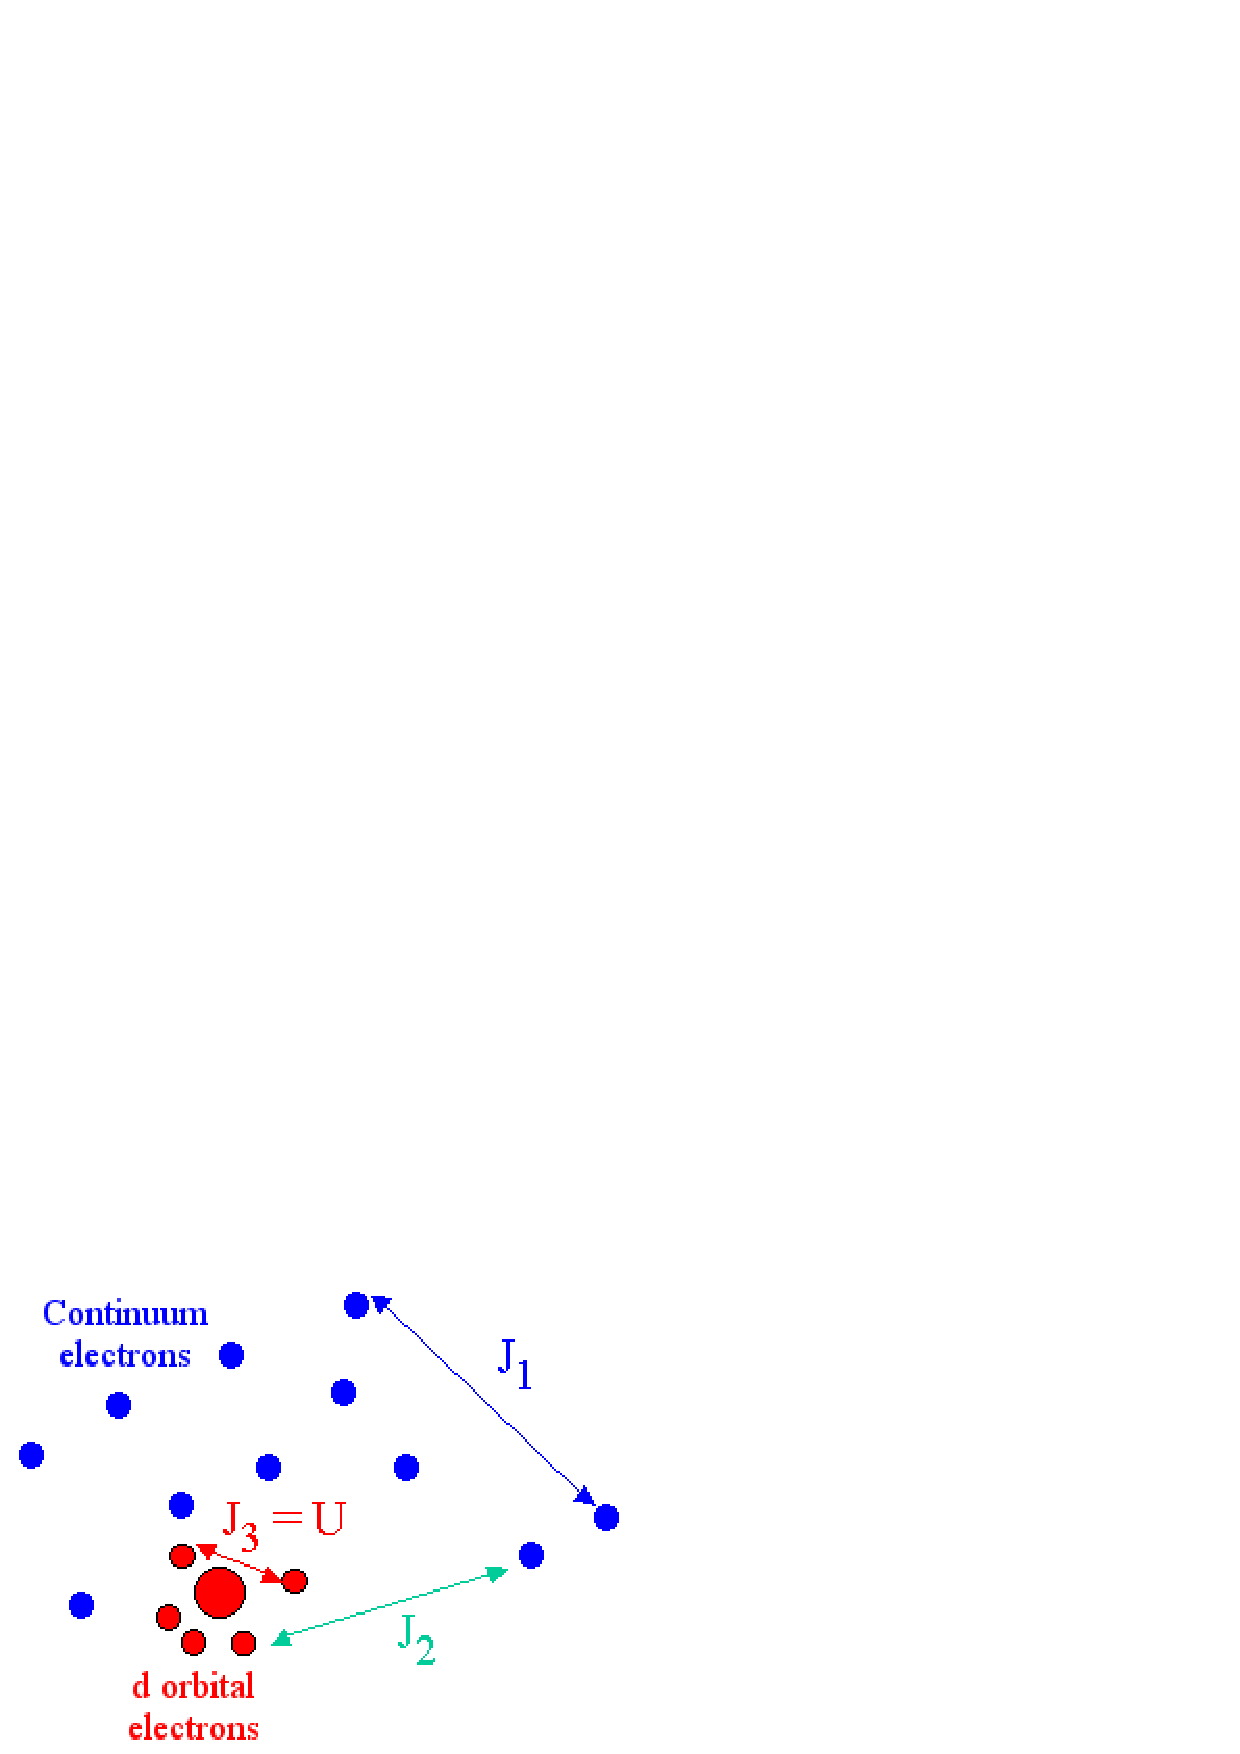
\includegraphics[width=6cm]{Pictures/ExchInt.png}
	\end{center}
	\caption{Carrier interaction with no change of the number of electron on the impurity, derived from the hamiltonian ${\cal H}_{Coulomb}$.}
	\label{HybridEner}
	\end{figure}

	Doing this transformation is an important step, since we are now able to use a Heisenberg type spin hamiltonian instead of a hamiltonian mixing wave function, in addition to having the same formalism to write both type of exchange interactions, with just a difference in the exchange constants $I_{kk'}^{ex}$ and $I_{kk'}^{hyb}$.

	Supposing the coupling occur between two electrons with a close $k$ ($k \simeq k'$), we can rewrite $I_{kk'}^{hyb}$ as:
	\begin{align}
		\begin{array}{rl}
			I_{kk'}^{hyb} &= 2|V_{kd}|^2 \dfrac{U}{(E_k - E_d)(E_k - (E_d + U)} \\
						&= -2|V_{kd}|^2 \dfrac{U}{(E_k - E_d)(E_d + U - E_k}
		\end{array}
	\end{align}
Looking ath the Fig.~\ref{HybridEner}, one can see that $U$ and $E_k - E_d$ are both positive, while $E_k - (E_d + U)$. Thus, $I_{kk'}^{hyb}$ is negative, and we see that, while exchange lead to a ferromagnetic coupling, hybridization lead to an anti-ferromagnetic one. Their will be a competition in the semiconductor between these two for every type of carrier.

	Reusing the hypothesis done on Sec.~\ref{BandStruct} of small $k$ value, and the value of $V_{kd}$ presented in Eq.~\ref{Vkd}, we can rewrite the exchange constant:
	\begin{align}
		I_{00, \{c,v\}}^{hyb} &= -2 \left(\frac{U}{(E_{\{c,v\}}(0) - E_d)(E_d + U - E_{\{c,v\}}(0))}\right) \int \mathrm{d}\mathbf{r} \Phi_r^* (\mathbf{r}) {\cal H}_1 \psi_0^{\{c,v\}} \\
		I_{00, \{c,v\}}^{ex} &= \int \mathrm{d}\mathbf{r} \mathrm{d}\mathbf{r}' \psi_0^{*\{c,v\}} (\mathbf{r}) \Psi_d^* \frac{e^2}{4\pi \varepsilon_0 |\mathbf{r}' - \mathbf{r}|\psi_0^{\{c,v\}} (\mathbf{r}) \Psi_d} (\mathbf{r})
	\end{align}
In the valence band, the semiconductor have the $p$ symmetry, as discussed in Sec.~\ref{BandStruct}. We then write $I_{pd}$ as the sum of the hybridization and the exchange contributions:
	\begin{align}
		I_{pd} =I_{00, v}^{hyb} +  I_{00, v}^{ex}
	\end{align}
In the conduction band, the orbital are $s$, and so we will write the interaction $I_{sd}$. However, since $s$ orbital have a spherical symmetry, there is no hybridization contribution. The expression is then pretty easy:
	\begin{align}
		I_{sd} = I_{00, c}^{ex}
	\end{align}

	Having define those, we can now rewrite the Hamiltonian of the interaction with one magnetic atom in the Heisenberg notation:
	\begin{align}
		{\cal H}_{SQ} = {\cal H}_0 + {\cal H}_{eh} + I_{sd} \bm{\upsigma}.\mathbf{S} + I_{pd} \mathbf{J}.\mathbf{S}
	\end{align}
Since a DMS contain a small percentage of magnetic atoms, we can write the hamiltonian of the full semiconductor by summing on their position. We finally get:
	\begin{align}
	\label{HDMS}
		\begin{array}{rlcccccc}
			{\cal H}_{DMS} &= {\cal H}_0 &+& {\cal H}_{eh} &+& \underbrace{\sum_i I_{sd} (\mathbf{R}_i) \bm{\upsigma}.\mathbf{S}_i} &+& \underbrace{\sum_i I_{pd} (\mathbf{R}_i) \mathbf{J}.\mathbf{S}_i} \\
							&= {\cal H}_0 &+& {\cal H}_{eh} &+& {\cal H}_{sd} &+& {\cal H}_{pd}
		\end{array}
	\end{align}

	This can be further simplified with two approximations. First, since conduction electron see a lot of different atomic site, we can we can work with the mean value of the magnetic atoms spins, $\langle\mathbf{S} \rangle$, instead of their individual value $\mathbf{S}_i$. This is the mean field approximation, the magnetic atoms being seen as a magnetic field. And for the same reason, we can consider the interaction with each site of the crystal multiplied by the probability $x$ of being occupied by a magnetic atom, instead of summing only on the magnetic atoms positions. This is the virtual crystal approximation. We can then rewrite:
	\begin{align}
		{\cal H}_{sd} = \sum_i I_{sd} (\mathbf{R}_i) \bm{\upsigma}.\mathbf{S}_i = x \sum_{\mathbf{R}} I_{sd} (\mathbf{R}) \bm{\upsigma}.\langle\mathbf{S} \rangle
	\end{align}
Projecting along the quantization axis, we just replace $\bm{\upsigma}.\langle\mathbf{S} \rangle$ by $\sigma_z \langle S_z \rangle$. Since the atoms are seen as a magnetic field, they induce a degeneracy lift $\Delta E_c$ between the two spin values of conduction electron, $|\sigma_z = \pm \dfrac{1}{2} \rangle$:
	\begin{align}
		\Delta E_c = N_0 x \alpha \sigma_z \langle S_z \rangle
	\end{align}
with $\alpha \propto I_{sd}^{00}$ the interaction constant between impurity and conduction band Bloch function at $\mathbf{k} = 0$, and $N_0$ the number of cell per volume.
	The same consideration can be done for valence band. Hh and lh are separated via their spin values: $|J_z = \pm \dfrac{3}{2} \rangle$ for hh, $|J_z = \pm \dfrac{1}{2} \rangle$ for lh. We then get:
	\begin{align}
		\Delta E_v = N_0 x \frac{\beta}{3} J_z \langle S_z \rangle
	\end{align}
with $\beta \propto I_{pd}^{00}$ the interaction constant between impurity and conduction band Bloch function at $\mathbf{k} = 0$.

		\subsection{Mn case}
		
		For the Mn, we will rewrite the hamiltonian the exchange interaction in the valence band $I_{pd}$ as $I_{hMn}$ and $I_{sd}$ in the conduction band as $I_{eMn}$, since we look at the interaction between an exciton and the Manganese atom. The hamiltonian \ref{HDMS} is the rewrited:
		\begin{align}
		\label{HMnDMS}
			{\cal H}_{DMS, Mn} &= {\cal H}_0 + {\cal H}_{eMn} + {\cal H}_{hMn}
		\end{align}

		Lorem ipsum dolor sit amet, consectetur adipiscing elit. Curabitur tortor quam, imperdiet quis facilisis sed, fringilla a quam. Cras ante odio, hendrerit ac ante nec, cursus imperdiet urna. Mauris convallis ultricies purus, nec condimentum erat bibendum vel. Aliquam erat volutpat. Pellentesque condimentum, eros a consequat accumsan, turpis sem euismod nisi, sed fringilla quam turpis sit amet erat. Mauris dictum odio sed nisi dapibus, et molestie mauris rutrum. Praesent convallis dolor in nibh blandit bibendum. Quisque sit amet arcu consectetur lorem luctus venenatis nec quis dui. Aliquam erat volutpat. Aenean auctor elit nec tristique dignissim. Nulla massa mi, efficitur semper ex id, pretium eleifend massa. Vivamus sit amet orci scelerisque, gravida est ut, vulputate odio.

	Curabitur eget ipsum egestas dui viverra suscipit. Cras aliquet lacus vitae erat finibus semper. Nulla pharetra eget urna vitae sodales. Nunc faucibus velit lacus, nec ornare eros aliquet quis. Donec a orci nec sem pulvinar ultricies sit amet ut arcu. Nullam id vehicula enim, at tincidunt velit. Duis vestibulum lorem a molestie fringilla. Nullam tincidunt semper placerat. Donec nibh sem, ornare eget cursus ac, luctus sit amet eros. Phasellus eget interdum nisi. Donec mollis risus id lectus fringilla, et commodo risus iaculis. Donec at lacus sed nibh posuere posuere sit amet eget sapien. In dignissim, enim sit amet convallis fermentum, lacus nulla gravida tortor, non facilisis ex nisl sit amet augue. Maecenas eu enim condimentum, consectetur ligula vel, tincidunt nisl. Nam laoreet dictum volutpat. Donec at erat venenatis, ultrices lorem ac, vestibulum neque.
	
		\subsection{Cr case\label{CrDMS}}
		
		For the Cr, we will rewrite the hamiltonian the exchange interaction in the valence band $I_{pd}$ as $I_{hCr}$ and $I_{sd}$ in the conduction band as $I_{eCr}$, since we look at the interaction between an exciton and the Chromium atom. The hamiltonian \ref{HDMS} is the rewrited:
		\begin{align}
		\label{HCrDMS}
			\begin{array}{rlcc}
				{\cal H}_{DMS, Cr} &= {\cal H}_0 &+& {\cal H}_{eCr} + {\cal H}_{hCr} \\
								&= {\cal H}_0 &+& {\cal H}_{c-Cr}
			\end{array}
		\end{align}
		
		Lorem ipsum dolor sit amet, consectetur adipiscing elit. Curabitur tortor quam, imperdiet quis facilisis sed, fringilla a quam. Cras ante odio, hendrerit ac ante nec, cursus imperdiet urna. Mauris convallis ultricies purus, nec condimentum erat bibendum vel. Aliquam erat volutpat. Pellentesque condimentum, eros a consequat accumsan, turpis sem euismod nisi, sed fringilla quam turpis sit amet erat. Mauris dictum odio sed nisi dapibus, et molestie mauris rutrum. Praesent convallis dolor in nibh blandit bibendum. Quisque sit amet arcu consectetur lorem luctus venenatis nec quis dui. Aliquam erat volutpat. Aenean auctor elit nec tristique dignissim. Nulla massa mi, efficitur semper ex id, pretium eleifend massa. Vivamus sit amet orci scelerisque, gravida est ut, vulputate odio.

	Curabitur eget ipsum egestas dui viverra suscipit. Cras aliquet lacus vitae erat finibus semper. Nulla pharetra eget urna vitae sodales. Nunc faucibus velit lacus, nec ornare eros aliquet quis. Donec a orci nec sem pulvinar ultricies sit amet ut arcu. Nullam id vehicula enim, at tincidunt velit. Duis vestibulum lorem a molestie fringilla. Nullam tincidunt semper placerat. Donec nibh sem, ornare eget cursus ac, luctus sit amet eros. Phasellus eget interdum nisi. Donec mollis risus id lectus fringilla, et commodo risus iaculis. Donec at lacus sed nibh posuere posuere sit amet eget sapien. In dignissim, enim sit amet convallis fermentum, lacus nulla gravida tortor, non facilisis ex nisl sit amet augue. Maecenas eu enim condimentum, consectetur ligula vel, tincidunt nisl. Nam laoreet dictum volutpat. Donec at erat venenatis, ultrices lorem ac, vestibulum neque.
		
		\subsection{Effect of the confinement\label{ExchIntQD}}
		
		Now that we established the basics of the interactions between carriers and magnetic atoms, we will do as we did in Sec.~\ref{e-hIntQD} and reduce the size of the studied semiconductor until reaching the quantum dot size and see how these interaction evolve with this reduction. Since both carriers and magnetic atom are now confine inside a small volume, the wave-functions have a bigger overlap and we can expect an increase of the exchange energies.

%		The simple picture of the interaction between the electron of the semiconductor we get in Sec.~\ref{ExchDMS} using the Hartree-Fock approximation is not enough to understand the emission spectrum we get from our quantum dots. We need to go more into details. For a few paragraphs, we go back considering a semiconductor without magnetic atoms. As shown in \cite{ExchSplitInteratomic}, we can treat the interaction between one electron in the conduction band and the $N-1$ electron of the valence band as an interaction between this electron and the corresponding hole, with an adding exchange interaction. We can then write the exchange hamiltonian in a Heisenberg form as:
%	\begin{align}
%	\label{ehExchHamil}
%		{\cal H}_{SC}^{exch} = I_{eh} \bm{\upsigma}.\mathbf{J}
%	\end{align}
%The matrix elements being:
%	\begin{align}
%		\langle e,h|{\cal H}_{SC}^{exch}| e', h' \rangle = \delta_{h,h'} \delta_{e, e'} (\epsilon_e - \epsilon_h) - K_{h'ee'h} + I_{eh'e'h}
%	\end{align}
%with $\epsilon_{e,h}$ the energy level of the electron and hole, $K_{h'ee'h}$ the direct Coulomb interaction and $I_{eh'e'h}$ the Coulomb exchange interaction.
%	\newline
%
%	[PLACEHOLDER]
%	\newline
	
	We will first consider the electron-hole exchange interaction in a QD without magnetic atom. Writing $\mathbf{J} = (J_z, J_+, J_-)$ with $J_+ = J_x + iJ_y$ and $J_- = J_x - iJ_y$, and $\bm{\upsigma} = (\sigma_z, \sigma_+, \sigma_-)$ with $\sigma_+ = \sigma_x + i\sigma_y$ and $\sigma_- = \sigma_x - i \sigma_y$, we can develop the hamiltonian \ref{ehExchHamil} in a QD symmetry:
	\begin{align}
	\label{Heh}
		\begin{array}{rll}
			{\cal H}_{e-h}^{exch} &= 2\delta_0 J_z \sigma_z &+ \dfrac{\delta_1}{2}\left(\exp (2i\varphi_1)j_+ \sigma_- - \exp (-2i\varphi_1)j_- \sigma_+ \right) \\
										& &+ \dfrac{\delta_2}{2}\left(\exp (2i\varphi_1)j_+ \sigma_+ + \exp (-2i\varphi_1)j_- \sigma_- \right)
		\end{array}
	\end{align}
with $\delta_0$ representing the splitting between dark and bright exciton, $\delta_1$ the splitting between the bright exciton states and $\delta_2$ the splitting between the dark exciton states. $\delta_0$ value is controlled both by long-range and short-range interaction, and is typically of about 1 meV in CdTe/ZnTe. $\delta_1$ only appear in anisotropic quantum dot, with $\varphi_1$ the direction of the anisotropy, and is induced by the long-range interaction, warying between a few tens and a few hundreds of $\mu$eV. Finally, $\delta_2$ primarily arise from the short-range interaction.
	
	Calculating the eigenstate of the hamiltonian \ref{Heh}, we find the optically active states are linearly polarized along $\varphi_1$ and $\varphi_1 + 90^{\circ}$ as followed:
	\begin{align}
		|\pi_{\varphi_1}\rangle = \frac{1}{\sqrt{2}}\left(\exp(-i\varphi_1)|+1\rangle + \exp(i\varphi_1)|-1\rangle\right) \\
		|\pi_{\varphi_1 + 90^{\circ}}\rangle = \frac{1}{\sqrt{2}}\left(\exp(-i\varphi_1)|+1\rangle - \exp(i\varphi_1)|-1\rangle\right)
	\end{align}

	In order to get the full image of the polarization, the VBM mixing presented in Sec.~\ref{VBM} should also be taken into account. Exchange interaction favours a linear emission along $\varphi_1$ and $\varphi_1 + 90^{\circ}$, while VBM orient the linear emission along $\theta$ and $\theta + 90^{\circ}$, as presented in Eq.~\ref{VBMPolar}. The competition between these two elements leads to an angle between the two different linearly polarized X lines different from $90^{\circ}$.
	\newline

	[PLACEHOLDER]
	\newline

	Curabitur eget ipsum egestas dui viverra suscipit. Cras aliquet lacus vitae erat finibus semper. Nulla pharetra eget urna vitae sodales. Nunc faucibus velit lacus, nec ornare eros aliquet quis. Donec a orci nec sem pulvinar ultricies sit amet ut arcu. Nullam id vehicula enim, at tincidunt velit. Duis vestibulum lorem a molestie fringilla. Nullam tincidunt semper placerat. Donec nibh sem, ornare eget cursus ac, luctus sit amet eros. Phasellus eget interdum nisi. Donec mollis risus id lectus fringilla, et commodo risus iaculis. Donec at lacus sed nibh posuere posuere sit amet eget sapien. In dignissim, enim sit amet convallis fermentum, lacus nulla gravida tortor, non facilisis ex nisl sit amet augue. Maecenas eu enim condimentum, consectetur ligula vel, tincidunt nisl. Nam laoreet dictum volutpat. Donec at erat venenatis, ultrices lorem ac, vestibulum neque.	


	\section{Fine and hyperfine structure of a magnetic atom in II-VI semiconductor}
	
	FINDING A WAY TO SPEAK ABOUT THE EFFECT OF VBM AS EXPLAIN IN CLAIRE THESIS~\cite{ClaireTh} p.30.
	
	\begin{figure}[h!]
	\begin{center}
		\includegraphics[width=10cm]{../FillingPicture.png}
	\end{center}
	\caption{Magnetic atom in a Zinc-Blend lattice}
	\label{MagAtInclusion}
	\end{figure}
	
		\subsection{Mn atom in II-VI semiconductor}

		Mn in a lattice -> modification of orbital -> spin-orbit interaction. Magnetic anisotropy + anisotropy of strain. (Mn has nuclear spin 5/2 -> hyperfine interaction?)
\newline
		
		Lorem ipsum dolor sit amet, consectetur adipiscing elit. Curabitur tortor quam, imperdiet quis facilisis sed, fringilla a quam. Cras ante odio, hendrerit ac ante nec, cursus imperdiet urna. Mauris convallis ultricies purus, nec condimentum erat bibendum vel. Aliquam erat volutpat. Pellentesque condimentum, eros a consequat accumsan, turpis sem euismod nisi, sed fringilla quam turpis sit amet erat. Mauris dictum odio sed nisi dapibus, et molestie mauris rutrum. Praesent convallis dolor in nibh blandit bibendum. Quisque sit amet arcu consectetur lorem luctus venenatis nec quis dui. Aliquam erat volutpat. Aenean auctor elit nec tristique dignissim. Nulla massa mi, efficitur semper ex id, pretium eleifend massa. Vivamus sit amet orci scelerisque, gravida est ut, vulputate odio.

	\begin{figure}[h!]
	\begin{center}
		\includegraphics[width=10cm]{../FillingPicture.png}
	\end{center}
	\caption{Mn fine and hyperfine structure}
	\label{MnFineHyperfines}
	\end{figure}

	Curabitur eget ipsum egestas dui viverra suscipit. Cras aliquet lacus vitae erat finibus semper. Nulla pharetra eget urna vitae sodales. Nunc faucibus velit lacus, nec ornare eros aliquet quis. Donec a orci nec sem pulvinar ultricies sit amet ut arcu. Nullam id vehicula enim, at tincidunt velit. Duis vestibulum lorem a molestie fringilla. Nullam tincidunt semper placerat. Donec nibh sem, ornare eget cursus ac, luctus sit amet eros. Phasellus eget interdum nisi. Donec mollis risus id lectus fringilla, et commodo risus iaculis. Donec at lacus sed nibh posuere posuere sit amet eget sapien. In dignissim, enim sit amet convallis fermentum, lacus nulla gravida tortor, non facilisis ex nisl sit amet augue. Maecenas eu enim condimentum, consectetur ligula vel, tincidunt nisl. Nam laoreet dictum volutpat. Donec at erat venenatis, ultrices lorem ac, vestibulum neque.
	
		\subsection{Cr atom in II-VI semiconductor\label{CrSemiCon}}
	
		As presented in Sec.~\ref{CrDMS}, the Chromium is included in CdTe as Cr$^2+$. This isotope has an electronic spin $S = 2$, an orbital momentum $L = 2$ and \emph{no nuclear spin}. Therefore, Cr presents in our sample no hyperfine structure. However, the non-nul orbital momentum shows that it presents a strong coupling to strain. The fine structure will the be of importance in the study of this atom.
		
	\begin{figure}[h!]
		\label{Jahn-Teller}
		\begin{center}
			\includegraphics[width=10cm]{../FillingPicture.png}
		\end{center}
		\caption{Atomic configuration in Jahn-Teller effect + three minima}
	\end{figure}

		Cr atoms are incorporated into II-VI semiconductors as Cr$^{2+}$ ions on cation sites forming a deep impurity level. This isotope presents \emph{no nuclear spin}, meaning we don't have to consider the hyperfine structure of a Cr atom in a II-VI semiconductor. The ground state of a free Cr$^{2+}$ is $^{5}$D with the orbital quantum number L=2 and a spin S=2 yielding a 25-fold degeneracy. In the crystal field of T$_{d}$ symmetry of the tetrahedral cation site in zinc-blende crystal, the degeneracy is partially lifted (see Fig.~\ref{CrinIIVI}): the $^{5}$D term splits into 15-fold degenerate orbital triplet $^{5}$T$_{2}$ and 10-fold degenerate orbital doublet $^{5}$E. The Jahn-Teller distortion reduces the symmetry to D$_{2d}$ and leads to a splitting of the $^{5}$T$_{2}$ ground state into a 5-fold degenerate $^{5}$B$_{2}$ orbital singlet and a $^{5}$E orbital doublet.
		\newline
		
		[DEVELOP ON JAHN-TELLER]
		\newline

		The ground state orbital singlet $^{5}$B$_{2}$ is further split by the spin-orbit interaction. In a strain free crystal, it was found that the ground state splitting can be described by the spin effective Hamiltonian ~\cite{VallinEPR}:
		\begin{align}
			\label{exchange}
			{\cal H}_{Cr,CF}=D_0S_z^2+\frac{1}{180}F[35S_z^2-30S(S+1)S_z^2+25S_z^2]+\frac{1}{6}a[S_1^4+S_2^4+S_3^4]
		\end{align}
with the Cr spin S=2 and $|D_0|\gg|a|$, $|F|$. In the model presented here, we use $a=0$ and $F=0$. The x, y, z principal axes were found to coincide with the cubic axes (1,2,3) giving rise to three identical sites, each given by \ref{exchange} but with the z axis of each along a different cubic axis (1,2,3). A value of D$_0\approx+30 \mu eV$ was estimated from Electron Paramagnetic Resonance (EPR) measurements in highly diluted bulk (Cd,Cr)Te~\cite{VallinEPR}.

		\begin{figure}[hbt]
			\label{CrinIIVI}
			\begin{center}
				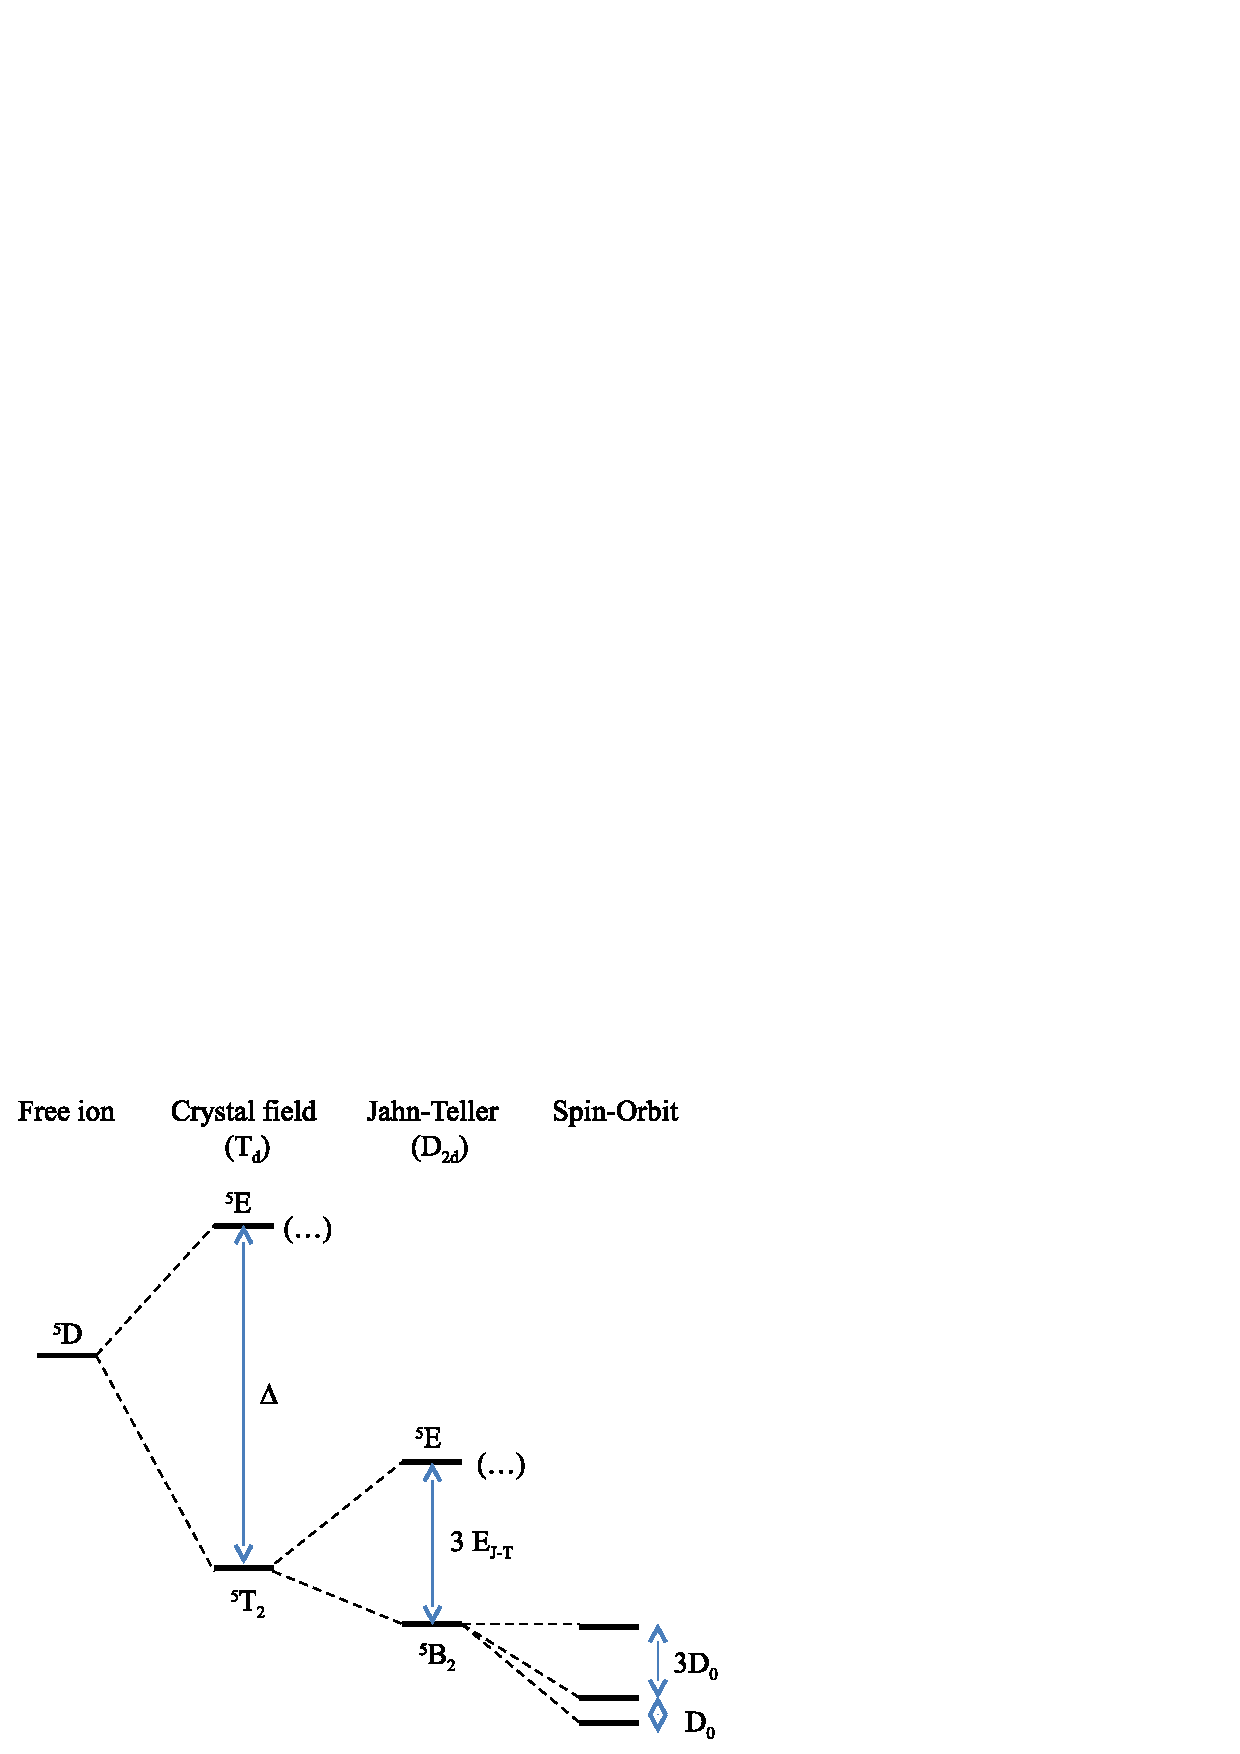
\includegraphics[width=7cm]{Pictures/CrinIIVI.png}
			\end{center}
			\caption{Scheme of the energy level splitting of Cr$^{2+}$ at a cation site in II-VI compounds having zinc blende structure (T$_d$) with a crystal field parameter $\Delta$, a Jahn-Teller energy E$_{J-T}$ and a spin-orbit level spacing D$_0$.}
		\end{figure}

		Static biaxial compressive strain in the (001) plane, as observed in self-assembled quantum dots, reduces the symmetry to D$_{2d}$ and destabilize the Cr $3d$ orbitals $d_{xz}$ and $d_{yz}$ having an electron density pointing along the $[$001$]$ axis ($z$ axis). The Cr ground state is then a 5-fold degenerated orbital singlet formed from the $d_{xy}$ orbital. It corresponds to the Jahn-Teller ground state with a tetragonal distortion along the $[$001$]$ axis~\cite{DefPonctSemiCon}.

		An applied stress will also  influence the Cr spin fine structure splitting through the modification of the crystal field and the spin-orbit interaction~\cite{VallinEPR}. For an arbitrary strain tensor, the general form of the Cr ground state spin effective Hamiltonian is
		\begin{align}
		\label{FullCrHamil}
			{\cal H}_{Cr,\varepsilon} = c_1 e_A S_{\theta} + c_2 e_{\theta} S_{\theta} + c_3 e_{\epsilon} S_{\epsilon} + c_4e_{\zeta} S_{\zeta} + c_5(e_{\xi} S_{\xi} + e_{\eta} S_{\eta})
		\end{align}
with $S_i$ defined as:
		\begin{align}
			\begin{array}{rl}
			\label{Svalues}
				S_{\theta} &= S_{z}^2  -\dfrac{1}{2} [S_{x}^2 + S_{y}^2] \\
				S_{\epsilon} &= \dfrac{1}{2} \sqrt{3} [S_{x}^2 - S_{y}^2] \\
				S_{\xi} &= S_{y} S_{z} + S_{z} S_{y} \\
				S_{\eta} & = S_{x} S_{z} + S_{z} S_{x} \\
				S_{\zeta} &=S_{x} S_{y} + S_{y} S_{x}
			\end{array}
		\end{align}
and $e_i$ defined similarly as:
		\begin{align}
			\begin{array}{rl}
			\label{evalues}
				e_{\theta} &= \varepsilon_{zz} - \dfrac{1}{2} [\varepsilon_{xx} + \varepsilon_{yy}] \\
				e_{\epsilon} &= \dfrac{1}{2} \sqrt{3}[\varepsilon_{xx} - \varepsilon_{yy}] \\
				e_{\xi} &= \varepsilon_{yz} + \varepsilon_{zy} \\
				e_{\eta} &= \varepsilon_{xz} + \varepsilon_{zx} \\
				e_{\zeta} &= \varepsilon_{xy} + \varepsilon_{yx} \\
				e_A &= \varepsilon_{xx} + \varepsilon_{yy} + \varepsilon_{zz}			
			\end{array}
		\end{align}

		As shown in Sec.~\ref{BPSec}, we can write for a flat self-assembled quantum dots with dominant large biaxial strain:
		\begin{align*}
			\varepsilon_{xx} = \varepsilon_{yy} = \varepsilon_{\parallel} \\
			\varepsilon_{zz}=-2\frac{C_{11}}{C_{12}}\varepsilon_{\parallel}
		\end{align*}
where C$_{11}\approx$ 5.4 10$^{10}Pa$ and C$_{12}\approx$ 3.7 10$^{10}Pa$ are the elastic constants of CdTe~\cite{CdTeElConst}. For this strain configuration, the Cr fine structure is controlled by the spin-lattice coupling coefficients $c_1$ (symmetric coefficient) and $c_2$ (tetragonal coefficients). Strain-coupling coefficients estimated from EPR measurements in bulk Cr doped CdTe are listed in table \ref{StrCouplCoef}.

		\begin{table}[htb] \centering
			\caption{Values for spin to strain coupling coefficients of Cr in bulk CdTe (in $meV$) extracted from ref.~\cite{VallinEPR}.\label{StrCouplCoef}}
			\renewcommand{\arraystretch}{1.0}
			\begin{tabular}{ccccc}
				\hline\hline
				$c_{1}$ & $c_{2}$ & $c_{3}$  & $c_{4}$  & $c_{5}$ \\
				-0.25$\pm$2 & +4.9 $\pm$2& -1.25$\pm$0.5 & +4.9$\pm$2 & +3.7$\pm$1.25 \\
				\hline\hline
			\end{tabular}
		\end{table}

		We can now simplify the hamiltonian \ref{FullCrHamil}, first reducing it to the active term in our case:
		\begin{align*}
			{\cal H}_{Cr,\varepsilon} &= c_1 e_A S_{\theta} + c_2 e_{\theta} + S_{\theta}
		\end{align*}
Replacing now $e_A$, $e_{\theta}$ and $S_{\theta}$ by their value given in \ref{Svalues} and \ref{evalues}, and using the equalities given in Sec.~\ref{BPSec}, we can rewrite the strain controlled part of the spin Hamiltonian as ${\cal H}_{Cr,\varepsilon}$, depending only on $\varepsilon_{\parallel}$:
		\begin{align}
			\begin{array}{rlcc}
			\label{HamilD0}
				{\cal H}_{Cr,\varepsilon_{\parallel}} &=& \underbrace{\dfrac{3}{2}\varepsilon_{\parallel}[2c_1(1-\dfrac{C_{12}}{C_{11}})-c_2(1+2\dfrac{C_{12}}{C_{11}})]} & S_z^2 \\
													&=& D_0 & S_z^2
			\end{array}
		\end{align}
where we can estimate D$_0\approx$ 1$\pm$0.6 meV from the values of the spin-strain coupling coefficients in CdTe (table \ref{StrCouplCoef}). However one should note the quantum dots could be partially relaxed and may contain a significant amount of Zn. We were not able to find spin to strain coupling coefficients for Cr in ZnTe and (Cd,Zn)Te alloy in literature. A value of D$_0\approx$+280$\mu$eV, much larger than for CdTe, was however estimated in strain-free Cr-doped bulk ZnTe~\cite{VallinEPR}. Larger spin-strain coupling coefficients could then expected for Cr in ZnTe and (Cd,Zn)Te alloys.

		Finally, an anisotropy of the strain in the quantum dot plane (001) with principal axis along $[$010$]$ or $[$100$]$ axes ($\varepsilon_{xx}\neq\varepsilon_{yy}$ and $\varepsilon_{xy}$=$\varepsilon_{yx}$=0) would affect the Cr fine structure through the tetragonal coefficient c$_3$. This coupling can be described by an additional term in the spin-strain Hamiltonian
		\begin{align}
			\begin{array}{rlcc}
			\label{HamilE}
				{\cal H}_{Cr,\varepsilon_{\perp}} &=& \underbrace{\dfrac{3}{4} c_3 (\varepsilon_{xx}-\varepsilon_{yy})} & (S_x^2 - S_y^2) \\
												&=& E & (S_x^2 - S_y^2)
			\end{array}
		\end{align}

		This anisotropy term E couples Cr spin states separated by two units and in particular S$_z$=+1 to S$_z$=-1 which are initially degenerated. It could be exploited to induce a large strain mediated coherent coupling between a mechanical oscillator and the Cr spin~\cite{SpinOsciCoupl}.
		
		We can now group \ref{HamilD0} and \ref{HamilE} in order to write the complete hamiltonian of anisolated Cr in a strained, anisotropic CdTe/ZnTe quantum dot:
		\begin{align}
			\begin{array}{lrccc}
				\label{Cralone}
				{\cal H}_{Cr,\varepsilon} &=& {\cal H}_{Cr,\varepsilon_{\parallel}} &+& {\cal H}_{Cr,\varepsilon_{\perp}} \\
										&=& D_0 S_z^2 &+& E(S_x^2 - S_y^2)
			\end{array}
		\end{align}
	
	
	\section{A simple example: the X-Mn system}
	
	Lorem ipsum dolor sit amet, consectetur adipiscing elit. Curabitur tortor quam, imperdiet quis facilisis sed, fringilla a quam. Cras ante odio, hendrerit ac ante nec, cursus imperdiet urna. Mauris convallis ultricies purus, nec condimentum erat bibendum vel. Aliquam erat volutpat. Pellentesque condimentum, eros a consequat accumsan, turpis sem euismod nisi, sed fringilla quam turpis sit amet erat. Mauris dictum odio sed nisi dapibus, et molestie mauris rutrum. Praesent convallis dolor in nibh blandit bibendum. Quisque sit amet arcu consectetur lorem luctus venenatis nec quis dui. Aliquam erat volutpat. Aenean auctor elit nec tristique dignissim. Nulla massa mi, efficitur semper ex id, pretium eleifend massa. Vivamus sit amet orci scelerisque, gravida est ut, vulputate odio.

	\begin{figure}[h!]
	\begin{center}
		\includegraphics[width=10cm]{../FillingPicture.png}
	\end{center}
	\caption{QD spectra 0 Mn, 1 Mn, 2 Mn}
	\label{MnSpectra}
	\end{figure}

	Curabitur eget ipsum egestas dui viverra suscipit. Cras aliquet lacus vitae erat finibus semper. Nulla pharetra eget urna vitae sodales. Nunc faucibus velit lacus, nec ornare eros aliquet quis. Donec a orci nec sem pulvinar ultricies sit amet ut arcu. Nullam id vehicula enim, at tincidunt velit. Duis vestibulum lorem a molestie fringilla. Nullam tincidunt semper placerat. Donec nibh sem, ornare eget cursus ac, luctus sit amet eros. Phasellus eget interdum nisi. Donec mollis risus id lectus fringilla, et commodo risus iaculis. Donec at lacus sed nibh posuere posuere sit amet eget sapien. In dignissim, enim sit amet convallis fermentum, lacus nulla gravida tortor, non facilisis ex nisl sit amet augue. Maecenas eu enim condimentum, consectetur ligula vel, tincidunt nisl. Nam laoreet dictum volutpat. Donec at erat venenatis, ultrices lorem ac, vestibulum neque.

	\begin{figure}[h!]
	\begin{center}
		\includegraphics[width=10cm]{../FillingPicture.png}
	\end{center}
	\caption{Mn energy level in a QD}
	\label{MnLevel}
	\end{figure}
		
	
\printbibliography

\end{document}